%!TEX program = xelatex
\documentclass[12pt,a4paper]{article}%titlepage表示标题单独页
\usepackage{ctex}%ctex套用英文标题格式(建议在英文论文混排中文时使用),ctexcap套用中文格式(等同于\documentclass{ctexart})
\renewcommand{\contentsname}{目录}
%\renewcommand{\figurename}{图}
%\renewcommand{\tablename}{表}
%\renewcommand{\thefigure}{\chinese{figure}}%将图片计数改为汉字数字
%\renewcommand{\thetable}{\chinese{table}}%将表格计数改为汉字数字
\usepackage[top=0.75in,bottom=0.75in,left=0.75in,right=0.75in]{geometry}%页边距设置
\usepackage[CJKbookmarks]{hyperref}%给pdf文档添加互动式链接和书签

\usepackage{amsmath,amssymb,esint}%数学公式类宏包;最末为积分符号拓展
\allowdisplaybreaks[0]%允许多行公式间换页,用//*表示不允许换页
\numberwithin{equation}{section}
\usepackage{bm}%加粗(用于vector)
%\usepackage{textcomp}%符号包,不能用于数学模式,建议不要和SIunits混用
%\usepackage[squaren]{SIunits}%科学单位包,可以用于数学模式(为了统一不要和textcomp混用),squaren选项消除和amssymb的冲突
\usepackage{graphicx}%插图宏包
%\usepackage{picinpar}%图文绕排
\usepackage{array}%表格宏包
%\usepackage{longtable}%长表格宏包
\usepackage{multicol}
\usepackage{extarrows}
%\usepackage{booktabs}%表格线宏包

%\usepackage[basic,box,gate,oldgate,ic,optics,physics]{circ}%电路图宏包
%\usepackage[normalem]{ulem}%下划线,删除线等宏包,参数表示不修改\emph{}格式
\usepackage[version=3]{mhchem}%化学宏包,包含mhchem和chemfig
%\usepackage[symbol]{footmisc}%脚注拓展,选项表示用符号做脚注记号

\renewcommand*{\vec}[1]{\bm{#1}}%矢量的格式,这里是加粗
\newcommand{\dif}{\mathrm{d}}
\newcommand{\diff}{\,\mathrm{d}}
\newcommand\mi{\mathrm{i}}
\newcommand\e{\mathrm{e}}%定义数学模式中常用的正体字符

%---------------------------------------
% 有空记得搜索和补充两处待补充内容
% 与倪军的课件相比, 主要的符号变动
% M 参照电磁学的习惯表示磁化强度 (单位体积)
% Debye 模型中一律统一到频率 \nu
% Einstein 函数, Debye 函数等使用花体表示
% 关于态数量的表示, 一律统一到 \Omega, 
%       连续正则分布中 \Omega, \Gamma 的含义对换
%------------------------------------

\begin{document}
\title{统计力学整理}
\author{吕铭 Lyu Ming}
\maketitle
\tableofcontents
\section{系统状态的量子描述} % (fold)
\label{sec:state_of_the_system}
\begin{enumerate}
    \item 微观状态: 
    系统内各粒子按量子态的一个分配方式
    \item  宏观状态: 
    系统内各粒子按能级的一个分布, 
    对应大量不同的微观状态 (源于能级简并)
    \item Boltzmann 等几率假设: 
    处平衡态的\emph{孤立系统}, 各可能\emph{微观状态}出现的几率相等
\end{enumerate}

% section state_of_the_system (end)
\section{系综理论} % (fold)
\label{sec:ensemble_theory}
\begin{enumerate}
    \item 统计系综 (ensemble): 大量微观结构相同, 
    处相同宏观条件的系统的集合. 若处平衡态, 称稳定系综
    \item 系综理论: 研究一定宏观条件下, 
    系统处在各微观状态的几率, 
    并将宏观量看作是对应微观量对系统一切可能微观状态的平均值, 
    即\emph{宏观量的统计平均值 $=$ 系综平均值 (各态历经假说)}
    \begin{itemize}
        \item 经典的情形: $\rho(q,p)\prod_i(\dif q_i\dif p_i)$, 
        其中分布函数 $\rho(q,p)$ 是归一化的
        \begin{equation}
            \overline B = \int\prod_i(\dif q_i\dif p_i)\rho(q,p)B(q,p)
        \end{equation}
        \item 量子的情形: $\rho_s, s = \{l,m,\cdots\}$ 
        系统处于微观态 $s$ 的几率
        \begin{equation}
            \overline B = \sum_s\rho_s B_s 
            = \operatorname{Tr}[\hat\rho\hat B]
        \end{equation}
    \end{itemize}
    \item 热力学第一定律的统计表达 $\dif U(y_1,y_2\cdots) = \dif Q + \dif W$, 其中
    \begin{align}
        &\dif W \equiv \sum_{i} Y_i\dif y_i 
        &\mbox{广义力: } Y_i = \sum_s\rho_s \frac{\partial E_s}{\partial y_i} \\
        &\dif Q \equiv \sum_s E_s\dif \rho_s
    \end{align}
    \item 热力学系统分类
    \begin{itemize}
        \item 孤立系统: 恒定的 $N, V, U$, 对应微正则 (Micro-Canonical) 系综
        \begin{itemize}
            \item 微正则分布: Boltzmann 等几率假设, 处平衡态的孤立系统, 各可能微观状态出现的几率相等
            \begin{equation}
                \rho_s = \frac 1\Omega
            \end{equation}
        \end{itemize}
        \item 封闭系统: 恒定的 $N, V, T$, 对应正则系综
        \begin{equation}
            \rho_s\propto\e^{-\beta E_s}
        \end{equation}
        \item 开放系统: 恒定的 $\mu, V, T$, 对应巨正则系综
        \begin{equation}
            \rho_{Ns}\propto\exp\left(-\alpha N -\beta E_s\right)
        \end{equation}
    \end{itemize}
    \item 熵的微观对应量: $-k\ln\rho$
    \begin{equation}
        S = -k\langle\ln\rho\rangle = -k\operatorname{Tr}[\hat\rho\ln\hat\rho]
    \end{equation}
\end{enumerate}
\subsection{正则系综} % (fold)
\label{sub:Canonical}
\begin{enumerate}
    \item 微观状态的正则分布: $\rho_s = Z^{-1}\e^{-\beta E_s}$. 对应于宏观状态的分布 $\rho_i = Z^{-1}\Omega(E_i)\e^{-\beta E_i}$ 
    \begin{itemize}
        \item 热力学 $\beta$:
        \begin{equation}
            \beta\equiv \frac{\partial\ln\Omega(E)}{\partial E} 
            = \frac 1{k_B} \frac{\partial S}{\partial E} 
            = \frac 1{k_BT}
        \end{equation}
        \item 量子表达 (正则密度矩阵)
        \begin{equation}
            \hat \rho_c = \frac 1Z\exp(-\beta \hat H)
        \end{equation}
        \item 广延性 $\ln Z = \ln Z^{(1)} + \ln Z^{(2)}$
        \item 偏离
        \begin{equation}
            \Omega\{n_i\} = \Omega\{(n_i)_m\}\exp\left[-\frac 12\sum_i(n_i)_m
            \left(\frac{\delta n_i}{(n_i)_m}\right)^2\right]
        \end{equation}
    \end{itemize}
    \item 配分函数 $Z$
    \begin{equation}
        Z(\beta,y) = \sum_s\e^{-\beta E_s(y)} = \sum_i \Omega(E_i)\e^{-\beta E_i}
    \end{equation}
    \item 热力学关系
    \begin{itemize}
        \item 内能
        \begin{equation}
            U = \frac 1Z\sum_s E_s\e^{-\beta E_s} 
            = -\frac 1Z \frac{\partial Z}{\partial \beta} 
            = -\frac{\partial\ln Z}{\partial \beta}
        \end{equation}
        \item 物态方程
        \begin{equation}
            Y_i = \sum_s \rho_s \frac{\partial E_s}{\partial y_i}
             = \sum_s \frac1{Z}\e^{-\beta E_s}\frac{\partial E_s}{\partial y_i}
             = -\frac 1\beta \frac{\partial\ln Z}{\partial y_i}
        \end{equation}
        如 $p = \beta^{-1}\partial\ln Z/\partial V$
        \item 熵
        \begin{equation}
            S = k_B\left(\ln Z + \beta E\right) 
            = k_B\left[\ln Z - \beta\frac{\partial \ln Z}{\partial \beta}\right]
        \end{equation}
        \item Helmholtz 自由能与化学势
        \begin{equation}
            F\equiv U-TS = -k_BT\ln Z,\quad
            \mu\equiv\left.\frac{\partial F}{\partial N}\right|_{y,T}
        \end{equation}
        \item Clausius 关系
        \begin{align}
            \dif Q &= \dif U - \sum_i Y_i\dif y_i 
            = -\dif\left(\frac{\partial\ln Z}{\partial \beta}\right) 
            + \frac 1\beta\left[\dif(\ln Z) - \frac{\partial\ln Z}{\partial \beta}\dif\beta\right] \nonumber \\
            &=\frac1\beta\dif\left(\ln Z - \beta\frac{\partial\ln Z}{\partial\beta}\right) = T\dif S
        \end{align}
        不可逆过程中 $Y_i'\ge Y_i$
    \end{itemize}
\end{enumerate}
\subsubsection{正则系综的连续形式} % (fold)
\label{ssub:canonical_continuous}
\begin{enumerate}
    \item 能量准连续条件下的正则分布
    \item $\Gamma$ 空间: 描述 $N$ 粒子总自由度 $f = N\gamma$ 的 $2f$ 维相空间. 其中系统处于 $\Gamma$ 空间中 $(q,p)$ 的几率密度
    \begin{equation}
        \rho(q,p)\diff^f q\dif^f p = \frac 1{N!h^f}\frac{\e^{-\beta E}}{Z}\diff^f q\dif^f p
    \end{equation}
    其中 $E = E(q,p,y)$, 配分函数 $Z$
    \begin{equation}
        Z = \frac1{N!h^f}\int\e^{-\beta E}\diff^f q\dif^f p
    \end{equation}
    改写为按能量分布的形式
    \begin{equation}
        \rho(E)\diff E = \frac 1Z \e^{-\beta E}\Omega(E)\diff E
    \end{equation}
    其中单位能量态密度
    \begin{equation}
        \Omega(E) = \frac 1{N! h^f} \frac{\dif}{\dif E}\int_{H(q,p)\le E}\dif^f q\dif^f p \equiv \frac 1{N! h^f} \frac{\dif\Gamma}{\dif E}
    \end{equation}
    \begin{itemize}
        \item 对于单原子理想气体 $\Gamma = V^N(2\pi mE)^{3N/2}/(3N/2)!$
        \item 最可几能量 $E_m$: 
        \begin{equation}
            \left.\frac{\dif\rho}{\dif E}\right|_{E_m} = 0 
            \Rightarrow \frac{\Omega'(E_m)}{\Omega(E_m)} = \beta
        \end{equation}
        特别的, 对于单原子理想气体, $E_m = (3N/2 - 1)k_BT \approx \overline E = 3Nk_BT/2$
    \end{itemize}
\end{enumerate}
% subsubsection canonical_continuous (end)
\subsubsection{广义能量均分原理} % (fold)
\label{ssub:general_equipartition}
原理: 设 $\xi$ 是 $E(q,p,y)$ 中的某一个广义坐标或广义动量, 在能量准连续近似下, 若 $E$ 在 $\xi$ 积分限上为 $\infty$, 则
\begin{equation}
    \left\langle\xi\frac{\partial E}{\partial\xi}\right\rangle = k_BT
\end{equation}

推论: 若 $\displaystyle E = \sum_{i=1}^nC_i\xi_i^l$, 则 $\displaystyle U = \overline E = \frac nl k_BT$
\begin{itemize}
    \item 非相对论理想气体 $E\propto p^2$, 因此 $U = 3Nk_BT/2$
    \item 极端相对论情形 $E\propto |p|$, $U = 3Nk_BT$
\end{itemize}
% subsubsection general_equipartition (end)
% subsection Canonical (end)
\subsection{巨正则系综} % (fold)
\label{sub:grand_canonical}
\begin{enumerate}
    \item 微观状态的巨正则分布 $\rho_{N,s} = \Xi^{-1}\exp(-\alpha-\beta E_s)$
    \item 巨配分函数
    \begin{equation}
        \Xi(\alpha,\beta, y) = \sum_{N=0}^\infty\sum_s\exp\left(-\alpha N - \beta E_s(y)\right)
         = \sum_N q^NZ_N
    \end{equation}
    其中 $q = \e^{-\alpha}$ 称为易逸度 (Fugacity), $Z_N$ 是 $N$ 粒子配分函数
    \begin{itemize}
        \item $\beta$ 同正则系综, $\alpha$
        \begin{equation}
            \alpha \equiv \frac{\partial \Omega(N,E)}{\partial N}
             = \frac 1{k_B}\frac{\partial S}{\partial N} = -\frac{\mu}{k_B T}
        \end{equation}
    \end{itemize}
    \item 热力学关系
    \begin{itemize}
        \item 平均粒子数 $\overline N$
        \begin{equation}
            \overline N = \frac 1\Xi\sum_N\sum_s N\e^{-\alpha N-\beta E_s} 
             = -\frac{\partial\ln\Xi}{\partial\alpha}
        \end{equation}
        \item 内能和物态方程与正则系综类似
        \begin{equation}
            U = -\frac{\partial\ln\Xi}{\partial\beta}\qquad
            Y = -\frac1\beta \frac{\partial\ln \Xi}{\partial y}
        \end{equation}
        \item 熵
        \begin{equation}
            S = k_B(\beta\overline E + \alpha\overline N + \ln\Xi) 
            = k_B\left(\ln\Xi - \alpha\frac{\partial\ln\Xi}{\partial\alpha} - \beta\frac{\partial\ln\Xi}{\partial\beta}\right)
        \end{equation}
        \item 巨热力学势
        \begin{equation}
            J \equiv U-TS-\mu N = -k_B T\ln\Xi
        \end{equation}
    \end{itemize}
\end{enumerate}
% subsection grand_canonical (end)
% section ensemble_theory (end)

\section{近独立粒子系统} % (fold)
\label{sec:independent_partical_system}
\begin{itemize}
    \item 平均意义下, 粒子间相互作用的能量 $\ll$ 单个粒子的能量
    \item 近独立粒子系统中仍然有粒子间相互, 作用使得系统能够达到平衡态
    \item 粒子即可以指实际粒子, 也可以指准粒子, 如声子, 旋子
    \item 独立性保证单粒子态有明确的含义, $E = \sum_i n_i\varepsilon_i$
    \item 原则上说以下三种分布均可以从任意一种系综导出
\end{itemize}
\subsection[Bose 统计]{Bose-Einstein 统计} % (fold)
\label{sub:bose_stat}
\begin{enumerate}
    \item 自旋是整数的粒子, 粒子不可分辨, 量子态容纳的粒子数不受限制
    \item 平衡态分布 (宏观状态): Bose 分布
    \begin{equation}
        n_i = \frac{\omega_i}{\exp(\alpha + \beta\varepsilon_i) - 1}
    \end{equation}
    微观状态与宏观状态的关系
    \begin{equation}
        \Omega\{n_i\} = \prod_i\frac{(n_i+\omega_i-1)!}{n_i!(\omega_i-1)!}
    \end{equation}
    \item 巨配分函数与单粒子巨配分函数
    \begin{equation}
        \Xi = \prod_i\Xi_i \qquad 
        \Xi_i = \left[1-\exp(-\alpha-\beta\epsilon_i)\right]^{-\omega_i}
    \end{equation}
\end{enumerate}
% subsection bose_stat (end)
\subsection[Fermi 统计]{Fermi-Dirac 统计} % (fold)
\label{sub:fermi_stat}
\begin{enumerate}
    \item 自旋半整数的粒子, 粒子不可分辨, 量子态容纳的粒子数最多一个
    \item 平衡态分布 (宏观状态): Fermi 分布
    \begin{equation}
        n_i = \frac{\omega_i}{\exp(\alpha + \beta\varepsilon_i) + 1}
    \end{equation}
    微观状态与宏观状态的关系
    \begin{equation}
        \Omega\{n_i\} = \prod_i\frac{\omega_i!}{n_i!(\omega_i-n_i)!}
    \end{equation}
    \item 巨配分函数与单粒子巨配分函数
    \begin{equation}
        \Xi = \prod_i\Xi_i \qquad 
        \Xi_i = \left[1+\exp(-\alpha-\beta\epsilon_i)\right]^{\omega_i}
    \end{equation}
\end{enumerate}
% subsection fermi_stat (end)
\subsection[Boltzmann (半经典) 统计]{Maxwell-Boltzmann 统计与半经典统计} % (fold)
\label{sub:boltzmann_stat}
\begin{enumerate}
    \item Boltzmann (半经典) 统计: 粒子 (不) 可以分辨, 量子态容纳的粒子数不受限制
    \item 平衡态分布 (宏观状态): Boltzmann 分布和半经典分布
    \begin{equation}
        n_i = \omega_i\e^{-\alpha-\beta\varepsilon_i}
    \end{equation}
    微观状态与宏观状态的关系: 
    \begin{equation}
        \Omega\{n_i\} = \frac{N!}{G}\prod_i \frac{\omega_i^{n_i}}{n_i!}
    \end{equation}
    Boltzmann 分布: $g = 1$, 半经典分布 $g = N!$
    \item 半经典分布是非简并条件下的 Bose/Fermi 分布
    \begin{equation}
        \e^\alpha\gg 1 \Longleftrightarrow \frac{n_i}{\omega_i}\ll 1 %为什么?
    \end{equation}
    \item 配分函数与单粒子配分函数
    \begin{equation}\label{equ:boltz_partition}
        Z = \frac{z^N}{g}\qquad z = \sum_s\e^{-\beta\varepsilon_s}
    \end{equation}
    \item 热力学量 (参加配分函数部分, 配合式(\ref{equ:boltz_partition}) 得到单粒子相关公式)
    \begin{itemize}
        \item 粒子数 $N = z\e^{-\alpha}$, 粒子数分布 $N_s = z^{-1}N\exp(-\beta\varepsilon_s)$
        \item 熵
        \begin{equation}
            S = Nk_B\left[\ln z - \beta\frac{\partial\ln z}{\partial\beta}\right] - k_B\ln g
        \end{equation}
        \item 化学势
        \begin{align}
            &\mbox{Boltzmann} && \mu = -k_B T\ln z \\
            &\mbox{半经典}    && \mu = -\alpha k_B T = -k_BT\ln\frac zN\label{equ:mu_semi_cla}
        \end{align}
    \end{itemize}
\end{enumerate}
% subsection boltzmann_stat (end)
\subsection{半经典近似} % (fold)
\label{sub:semi-classical_approx}
半经典近似的方法原则上并不局限于独立粒子近似 (如 \ref{ssub:canonical_continuous} 节), 以下讨论近独立粒子的情形.
\begin{enumerate}
    \item 近似条件: 能量准连续 $\Delta\varepsilon_i\ll k_B T$
    \footnote{这个近似条件是充分非必要的, 如 Fermi 气体中 (\ref{sub:fermi_gas}节) 中 $T\to 0$. 实际上只要求平均量子数较大即可.}. 
    并不要求非简并的, 如
    弱简并量子气体 (\ref{sub:degenerate_quantum_gas} 节), 
    BEC (\ref{sub:BEC} 节), 
    光子气体 (\ref{sub:photon_gas} 节), 
    Fermi 气体 (\ref{sub:fermi_gas} 节)
    \item 使用半经典的方法描述粒子状态和计算配分函数
    \begin{itemize}
        \item $\mu$ 空间: 经典体系中由广义坐标 $\{q_i\}_{i=1}^\gamma$ 与广义动量 $\{p_i\}_{i=1}^\gamma$ 构成的 $2\gamma$ 维相空间.
        $\gamma$ 为粒子自由度
        \item 极限定理: 大量子数的状态在 $\mu$ 空间对应 $h^\gamma$ 的相体积
        \item 单粒子配分函数: 
        \begin{equation}
            z = \frac 1{h^\gamma}\int\dif\omega\exp(-\beta\varepsilon),\qquad
            \dif\omega = \prod_{i=1}^\gamma \dif p_i\dif q_i
        \end{equation}
        \item 能态密度 $\sum_s f_s = \sum_i f(\varepsilon_i) = \int g(\varepsilon)f(\varepsilon)\dif\varepsilon$
        \begin{equation}
            g(\varepsilon) = \frac1{h^{\gamma}}\frac{\dif}{\dif\varepsilon}\int_{\le\varepsilon}\dif\omega
        \end{equation}
        \begin{itemize}
            \item 一维谐振子: $g(\varepsilon) = 1/\hbar\omega$
            \item 二维谐振子: $g(\varepsilon) = \varepsilon/(\hbar\omega)^2$
            \item 三维转子: $g(\varepsilon) = 2I/\hbar^2$
            \item 三维空间单原子分子 (非相对论): 
            \begin{equation}\label{equ:state_density_for_ideal_gas}
                g(\varepsilon) = 2\pi V\left(\frac{2m}{h^2}\right)^{3/2}g_s\sqrt\varepsilon
            \end{equation}
            其中 $g_s = 2s+1$ 为自旋因子
        \end{itemize}
    \end{itemize}
\end{enumerate}
% subsection semi-classical_approx (end)
% section independent_partical_system (end)

\section{理想气体类模型} % (fold)
\label{sec:ideal_gas_like_model}
\subsection{经典理想气体} % (fold)
\label{sub:ideal_gas}
\begin{enumerate}
    \item 半经典近似, 非简并条件, 考虑相互独立的质心平动与内部运动
    \begin{equation}
        \varepsilon_{i,t} = \varepsilon_t + \varepsilon_i, \qquad
        \omega_{i,t} = \omega_t\omega_i,\qquad
        z(\beta,V) = z_t(\beta, V)z_i(\beta)
    \end{equation}
    \item 平动配分函数
    \begin{equation}
        z_t = h^{-3} V\int\dif^3p\exp\left[\frac\beta{2m}(p_x^2+p_y^2+p_z^2)\right]
        =\frac{V}{\lambda_T^3}
    \end{equation}
    其中 $\lambda_T\equiv h/\sqrt{2\pi mk_BT}$ 是与 $k_BT$ 对应的 de Brogie 波长
    \begin{itemize}
        \item 非简并条件
        \begin{equation}
            \e^\alpha \gg 1 \Longleftrightarrow 
            \frac zN =  \frac 1{n\lambda_T^3} \gg 1
        \end{equation}
        \begin{itemize}
            \item 非简并条件即 $\lambda_T \ll n^{-1/3}$, 波长远小于粒子平均间距
        \end{itemize}
    \end{itemize}
    \item 内部自由度: 振动 (一维谐振子为例)
    \begin{itemize}
        \item 能量 $\varepsilon_\nu = \left(n+1/2\right)h\nu$, 
        特征温度 $\theta_\nu\equiv h\nu/k_B\sim 10^3\mathrm K$
        \item 配分函数
        \begin{equation}
            z_\nu = \sum_{n=0}^\infty\exp\left[-\beta\left(n+\frac12\right)h\nu\right]
            =\frac{\exp\left(-\theta_\nu/2T\right)}{1-\exp\left(-\theta_\nu/T\right)}
        \end{equation}
        \item 能量
        \begin{equation}
            E_\nu =-N \frac{\partial\ln z_v}{\partial\beta} 
            = Nh\nu\left[\frac 12 + \frac{\exp(-\beta h\nu)}{1-\exp(-\beta h\nu)}\right]
        \end{equation}
        \item 热容量
        \begin{equation}
            C_V^{(\nu)} = \left(\frac{\partial E_\nu}{\partial T}\right)_V 
            = nk_B\mathcal E\left(\frac{\theta_\nu}T\right)
        \end{equation}
        其中 Einstein 函数定义
        \begin{equation}\label{equ:einstein_func}
            \mathcal E(x) \equiv \frac{x^2\exp(x)}{(1-\exp(x))^2}
        \end{equation}
        \begin{itemize}
            \item 低温极限: $C_V^{(\nu)}= Nk_B(\theta_\nu/T)^2\exp(-\theta_\nu/T)$, 对于系统热容贡献很小
            \item 高温极限: $z_\nu = T/\theta_\nu$, $E_\nu = Nk_B T$ (能量均分)
        \end{itemize}
    \end{itemize}
    \item 内部自由度: 转动
    \begin{itemize}
        \item 能量 $\varepsilon_r = \hbar^2 l(l+1)/2I$, 
        简并度 $\omega_r = 2l+1$, 
        特征温度 $\theta_r = \hbar^2/(2Ik_B)\sim 10^1\mathrm K$
        \item 配分函数
        \begin{equation}
            z_r = \sum_{l=0}^\infty (2l+1)\exp\left[-\frac{\theta_r}T l(l+1)\right]
        \end{equation}
        \begin{itemize}
            \item 低温极限: $C_V^{(r)} = 12Nk_B(\theta_r/T)^2\exp\left(-2\theta_r/T\right)$
            \item 高温极限: $z_r = T/\theta_r$, $E_r = Nk_B T$ (能量均分)
        \end{itemize}
    \end{itemize}
    注意, 高 (低) 温极限是相对于特征温度的. 一般情况下, 随着温度上升, 平动, 转动, 振动依次被激发
    \item 特别的, 对于单原子理想气体, $z_i = g_s = \mbox{const.}$, $z = g_sV/\lambda_T^3$
        \begin{align}
            &U = -N \frac{\partial \ln z_t}{\partial \beta} 
            = \frac 32 Nk_B  T &&\mbox{(能量均分)} \\
            &C_V = \left(\frac{\partial E}{\partial T}\right)_V 
            = \frac 32 Nk_B \\
            &p = \frac N\beta \frac{\partial\ln z_t}{\partial V}
            =nk_BT &&\mbox{理想气体状态方程} \\
            &S =  Nk_B\left(\ln\frac{g_s}{n\lambda_T^3} + \frac 52\right)\\
            &\mu = k_BT\ln\frac{n\lambda_T^3}{g_s}
        \end{align}
\end{enumerate}
% subsection ideal_gas (end)
\subsection{弱简并量子气体} % (fold)
\label{sub:degenerate_quantum_gas}
\begin{enumerate}
    \item 半经典近似, 弱简并条件 ($n\lambda_T^3 < 1$) 
    讨论 $n\lambda_T^3$ 展开高次项的量子效应, 其中
    \begin{equation}
        \lambda_T = \sqrt{\frac{\beta h^2}{2\pi m}}\propto\frac 1{\sqrt{mT}}
    \end{equation}
    温度越低, 粒子质量越小, 体系粒子数密度越大, 量子修正项也越大
    \item 平衡态分布
    \begin{equation}
        n_i = \frac{\omega_i}{\exp(\alpha+\beta\varepsilon_i)\pm 1}
        \left\{\begin{array}{ll}
        + &\mbox{Fermi} \\
        - &\mbox{Bose}
        \end{array}\right.
    \end{equation}
    \item 巨配分函数
    \begin{equation}
        \Xi =\prod_i \left(1\pm\e^{-\alpha-\beta\varepsilon_i}\right)^{\pm\omega_i}
        = \prod_i\Xi_i
    \end{equation}
    \item 半经典近似下的 $\ln\Xi$
    \begin{align}
        \ln\Xi &= \pm\sum_i\omega_i\ln\left(1\pm\e^{-\alpha-\beta\epsilon_i}\right) 
        = \pm\int_0^\infty g(\varepsilon)\ln\left(1\pm\e^{-\alpha-\beta\epsilon}\right)\dif\varepsilon \nonumber\\
        &= \pm CV\int_0^\infty \sqrt\varepsilon\ln\left(1\pm\e^{-\alpha-\beta\epsilon}\right)\dif\varepsilon 
        = \frac{Vg_s}{\lambda_T^{3}}\sum_{i=1}^\infty(\mp)^{i-1}i^{-5/2}\e^{-i\alpha}
    \end{align}
    其中 $g(\varepsilon)$ 参见式(\ref{equ:state_density_for_ideal_gas}), 系数 $C = 2\pi g_s (2m)^{3/2} h^{-3}$\\
    由 $N = -\partial\ln\Xi/\partial\alpha$ 反解出 $\alpha$ 
    \begin{equation}
        \alpha = -\ln\frac{n\lambda_T^3}{g_s} \mp 2^{-3/2}\frac{n\lambda_T^3}{g_s} + \cdots
    \end{equation}
    代入可得
    \begin{equation}
        f(\alpha) \equiv \sum_{n=1}^\infty(\mp)^{n-1}n^{-5/2}\e^{-n\alpha} 
        = \frac{n\lambda_T^3}{g_s}\left(1\pm 2^{-5/2}\frac{n\lambda_T^3}{g_s}+\cdots\right)
    \end{equation}
    \item 宏观量
    \begin{align}
        &U = -\left(\frac{\partial\ln\Xi}{\partial\beta}\right)_{\alpha, V}
        =\frac 32\frac{\ln\Xi}\beta 
        = \frac 32 Nk_B T\left(1\pm 2^{-5/2}\frac{n\lambda_T^3}{g_s} + \cdots\right)\\
        &C_V = \left(\frac{\partial U}{\partial T}\right)_V 
        = \frac 32Nk_B \left(1\mp 2^{-7/2}\frac{n\lambda_T^3}{g_s} + \cdots\right) \label{equ:cv_for_quantum_gas}\\
        &p = \frac 1\beta \left(\frac{\ln\Xi}{\partial V}\right)_{\alpha,\beta} 
        = \frac {2U}{3V} = nk_B T\left(1\pm 2^{-5/2}\frac{n\lambda_T^3}{g_s} + \cdots\right)\\
        &S = k_B\left(\ln\Xi - \alpha\frac{\partial\ln\Xi}{\partial\alpha} - \beta\frac{\partial\ln\Xi}{\partial\beta}\right) 
        = Nk_B\left(\ln\frac{g_s}{n\lambda_T^3} + \frac 52 \pm 2^{-7/2}\frac{n\lambda_T^3}{g_s} + \cdots \right) \\
        &\mu = -\frac{\alpha}{\beta} = k_BT\left(\ln\frac{n\lambda_T^3}{g_s} \pm 2^{-3/2}\frac{n\lambda_T^3}{g_s} + \cdots\right)
    \end{align}
    \begin{itemize}
        \item Fermi 气体的能量, 熵, 压强比半经典的情况大, Bose 气体反之. 
        这来源于交换对称性导致的费米子相互吸引, 玻色子相互排斥
    \end{itemize}
\end{enumerate}
% subsection degenerate_quantum_gas (end)
\subsection{光子气体} % (fold)
\label{sub:photon_gas}
\begin{enumerate}
    \item 研究空腔黑体辐射的粒子观点. 理想简并 Bose 气体, $g_s = 2$
    \item 光子数不守恒: 不引入 $\alpha$ (Lagrange 乘子的观点) 
    或者 $\alpha\propto\mu = 0$ (恒定体积, 温度下 $F$ 取到极值) 
    于是光子数分布
    \begin{equation}
        n_i = \frac{\omega_i}{\e^{\beta\varepsilon_i} - 1} \Leftrightarrow
        n(\nu)\diff\nu = \frac{g(\nu)\diff\nu}{\e^{\beta h\nu} - 1}
    \end{equation}
    \item 态密度 (半经典近似)
    \begin{equation}
        \int g(\nu)\diff\nu = \frac{g_s}{h^3}\int\dif^3q\dif^3p 
        \Rightarrow g(\nu)\diff\nu = \frac{8\pi V}{c^3}\nu^2\diff\nu
    \end{equation}
    \item 辐射能量按频率分布: Planck 辐射公式
    \begin{equation}
        E(\nu)\diff\nu = n(\nu) h\nu\diff\nu 
        = \frac{8\pi V}{c^3}\frac{h\nu^3\diff\nu}{\e^{h\nu/k_BT} - 1}
    \end{equation}
    \begin{itemize}
        \item 低频高温极限 $h\nu\ll k_BT$: Rayleigh-Jeans 公式
        \begin{equation}
            E(\nu)\diff\nu =\frac{8\pi V}{c^3}k_BT\nu^2\diff\nu
        \end{equation}
        与经典电磁理论和 Boltzmann 统计的结果一致
        \item 高频低温极限 $h\nu\gg k_BT$: Wien 公式
        \begin{equation}
            E(\nu)\diff\nu = \frac{8\pi V}{c^3}h\nu^3\e^{-h\nu/k_BT}\diff\nu
        \end{equation}
        \item 辐射场总能量密度
        \begin{equation}\label{equ:photon_totE}
            u = \frac 1V\int_0^\infty E(\nu)\diff\nu 
            = \frac{8\pi^5k_B^4}{15h^3c^3}T^4
        \end{equation}
        \item 辐射通量密度: Stefan-Boltzmann 定律
        \begin{equation}
            J = \frac 1{4\pi}\int cu\cos\theta \diff\Omega
            = \frac c4 u \equiv \sigma T^4
        \end{equation}
        其中 Stefan 常量 $\sigma = \frac{2\pi^5k_B^4}{15h^3c^3}$
        \item 测量 Planck 常量 $h$: 测能量密度-波长极值
    \end{itemize}
    \item 巨配分函数 $\ln\Xi$
    \begin{equation}
        \ln\Xi(\beta, V) = -\int_0^\infty g(\nu)\ln(1-\e^{-\beta h\nu})\diff\nu 
        = \frac{8\pi^5 V}{45h^3c^3\beta^3}
    \end{equation}
    \item 热力学量
    \begin{align}
        &U = -\left(\frac{\partial\ln\Xi}{\partial\beta}\right)_{\alpha, V}
        = \frac{8\pi^5 V}{15h^3c^3\beta^4}
        \equiv bVT^4 &\mbox{同式(\ref{equ:photon_totE})}\\
        &C_V = \left(\frac{\partial U}{\partial T}\right)_V = 4bVT^3 \\
        &p = \frac 1\beta \left(\frac{\ln\Xi}{\partial V}\right)_{\alpha,\beta} 
        = \frac {U}{3V} = \frac 13 bT^4 \\
        &S = k_B\left(\ln\Xi - \beta\frac{\partial\ln\Xi}{\partial\beta}\right) 
        = 4k_B\ln\Xi = \frac 43 bVT^3 \\
        &G = U - TS + pV = 0 \Rightarrow \mu=0 &\mbox{光子数不守恒}
    \end{align}
\end{enumerate}
% subsection photon_gas (end)
\subsection{Einstein 晶体振动模型} % (fold)
\label{sub:einstein_solid}
\begin{enumerate}
    \item 三维 $N$ 个粒子, $3N$ 个简正模, 近似取作相同频率 $\nu$
    \item 配分函数 $z = \exp(-\beta h\nu/2)/(1-\exp(-\beta h\nu))$
    \item 能量 $E = 3Nh\nu/(\e^{\beta h\nu}-1) + E_0$
    \item 热容 $C_V = 3Nk_B\mathcal E(\theta_E/T)$, 其中特征温度 $\theta_E = h\nu/k_B$
    \begin{itemize}
        \item 高温极限 $C_V = 3Nk_B$ (能量均分)
        \item 低温极限 $C_V = 3Nk_B(\theta_E/T)^2\exp(-\theta_E/T)$, , 与实验定性相符, 定理不符
    \end{itemize}
    \item 从声子的观点看, 巨配分函数
    \begin{equation}
        \ln\Xi = -3N\ln\left(1-\e^{-\beta h\nu}\right)
    \end{equation}
\end{enumerate}
% subsection einstein_solid (end)
\subsection{Debye 模型与声子气体} % (fold)
\label{sub:debye_model}
\begin{enumerate}
    \item 将简谐振动中 $\varepsilon_\nu = h\nu(n+1/2)$ 视作 $n$ 个声子的能量, 各简正模独立振动, 声子彼此不可区分, 且 $n\ge 0$, 因而声子模型是粒子数不守恒的理想 Bose 气体
    \begin{equation}
        n_i = \frac{\omega_i}{\e^{\beta h\nu_i} - 1}
    \end{equation}
    \begin{itemize}
        \item 固体中粒子相互作用强, 不能直接用哪个近独立粒子统计, 
        但低温时简谐近似成立, 各简正模式相互独立, 因而声子是近独立的
        \item 声子是准粒子, 是关于振动激发的一种等效, 具有能量和动量. 
        不同于一般的粒子, 只存在于晶格中, 
        色散关系 ($\varepsilon$--$p$ 关系) 也不同
        \item 讨论实际固体比热时
        \begin{itemize}
            \item 金属在低温时表现出显著的自由电子气偏离
            \item 化合物分子间振动 (声频) 使用 Debye 模型
            \item 化合物分子内振动 (光频) 使用 Einstein 模型
        \end{itemize}
    \end{itemize}
    \item Debye 模型: $\lambda = v/\nu \ll$原子间距 时, 将振动频率视为 $0$--$\nu_D$ 的连续谱, 其中 $\nu_D$ 称为 Debye 频率
    \item 声子的描述: $\varepsilon = h\nu = vp$, $p = h\nu/v$
    \item 状态数: 
    \begin{equation}
        g(\nu)\diff\nu = 4\pi V\left(v_l^{-3} + 2v_t^{-3}\right)\nu^2\diff\nu \equiv B\nu^2\diff\nu\quad (0\le\nu\le\nu_D)
    \end{equation}
    其中包含一种纵波振动模式(声速 $v_l$), 两种横波振动模式(声速$v_t$)
    \item Debye 频谱: 总的简正模数量为 $3N$ 可以解得
    \begin{equation}
        g(\nu) = \begin{cases}
        \frac{9N}{\nu_D^3}\nu^2 &0\le\nu\le\nu_D \\
        0                     &\nu >\nu_D
        \end{cases}
    \end{equation}
    其中 $\nu_D = (9N/B)^{1/3}$, 据此得到 $\lambda_D \approx (4\pi V/3N)^{1/3}$ 与晶格间距同量级, 故模型是合理的
    \item Debye 温度: Debye 模型的特征温度 $\theta_D = h\nu_D/k_B\sim 200$K
    \item 能量与热容
    \begin{align}
        &U = U_0 + \int_0^{\nu_D}\frac{9N}{\nu_D^3}\frac{h\nu^3}{\exp(\beta h\nu) - 1}\diff\nu 
        = U_0 + 3Nk_BT\mathcal D(y_D) \\
        &C_V = \frac{9Nk_B}{\omega_D^3}\int_0^{\omega_D} \omega^2\mathcal E(\beta h\nu)\diff\nu 
        = 3Nk_B\left(4\mathcal D(y_D) - \frac{3y_D}{e^{y_D} - 1}\right)
    \end{align}
    其中 $y_D = \theta_D/T$, $\mathcal E(x)$ 是 Einstein 函数, 见式(\ref{equ:einstein_func}), $\mathcal D(y_D)$ 是 Debye 函数
    \begin{equation}\label{equ:debye_func}
        \mathcal D(y_D) = \frac 3{y_D^3}\int_0^{y_D}\frac{x^3}{e^x-1}\diff x
    \end{equation}
    \begin{itemize}
        \item 高温极限 $y_D\ll 1$: $C_V = 3Nk_B$ (能量均分)
        \item 低温极限 $y_D\gg 1$: $C_V = (12\pi^2/5)Nk_B(T/\theta_D)^3$, 
        与光子气类似
    \end{itemize}
    \item 物态方程
    \begin{align}
        &\ln\Xi(\beta,V) = -\int_0^{\nu_D}\frac{9N}{\nu_D^3}\nu^2\ln(1-\e^{-\beta h\nu})\diff\nu \\
        &p = \frac 1\beta\frac{\partial\ln\Xi}{\partial V} 
        = \frac{3N}{V\nu_D^3}\int_0^{\nu_D}\frac{h\nu^3}{\e^{\beta h\nu}-1}\diff\nu = \frac{U-U_0}{3V}
    \end{align}
    由于存在截断, 无法写出前面这样解析的各个宏观量
\end{enumerate}
% subsection debye_model (end)
\subsection{Bose-Einstein 凝聚} % (fold)
\label{sub:BEC}
\begin{enumerate}
    \item 简并 Bose 气体在临界温度 $T_c$ 以下的凝聚 (condensation) 现象
    \item 用化学式表达的粒子数 (以下定义基态 $\varepsilon_0 = 0$, 于是 $\mu<0$)
    \begin{equation}\label{equ:bec_N}
        N = \sum_i\frac{\omega_i}{\exp(\beta\varepsilon_i + \alpha) - 1} 
         = \sum_i\frac{\omega_i}{\exp[\beta(\varepsilon_i - \mu)] - 1}
    \end{equation}
    \item 临界温度: 由式(\ref{equ:bec_N}) 恒定 $N$ 时, $T$ 与 $\mu$ 负相关. 
    定义 $T_c : \mu(T \to T_c) \to 0$, 半经典近似下有下式, 计算参见式(\ref{equ:bose})
    \begin{equation}
        N = CV\int_0^\infty\dif\varepsilon\sqrt\varepsilon\left(\e^{\varepsilon/(k_B T_c)} - 1\right)^{-1}
        =CV(k_B T_c)^{3/2}\times\frac{\sqrt\pi}2\times2.612
    \end{equation}
    解得临界温度
    \begin{equation}\label{equ:tc_for_bec}
        T_c = \frac{h^2}{2\pi mk_B}\left(\frac{n}{2.612g_s}\right)^{2/3} = \left(\frac{n\lambda_T^3}{2.612g_s}\right)^{2/3}T
    \end{equation}
    \item 凝聚: $T\le T_c$ 时, $\omega_i(\exp[\beta(\varepsilon_0-\mu)]-1)^{-1}\to\infty$, 
    此时能量准连续的 $g(\varepsilon)\propto\sqrt\varepsilon$ 忽略基态不再适用 
    (据此也课件前面凝聚时 $\mu = 0$ 是在近似的). 
    基态粒子数
    \begin{equation}
        N_{\varepsilon = 0} = N\left[1-\left(\frac T{T_c}\right)^{3/2}\right]
    \end{equation}
    基态占据了宏观可计的粒子, 称为 Bose-Einstein 凝聚, 
    这是 $|\vec p| = 0$, 动量空间的凝聚
    \item 凝聚后的宏观性质
    \begin{itemize}
        \item $\varepsilon = 0$ 粒子的贡献: $U$, $p$, $\mu$, $S$ 均为 $0$; 
        起粒子源的作用
        \item $\varepsilon > 0$ 粒子事实上相当于 $\mu=0$ (即 $\alpha = 0$) 的开放系统
        \begin{equation}
            \ln\Xi|_{\varepsilon>0} = -CV\int_0^\infty\dif\varepsilon\sqrt\varepsilon\ln\left(1-\e^{-\beta\varepsilon}\right)
            =\frac{\sqrt\pi}2 CV\beta^{-3/2}\times1.341
        \end{equation}
        相关宏观量
        \begin{align}
            &U = -\frac{\partial\ln\Xi|_{\varepsilon>0}}{\partial\beta}
            = 1.783 CV\beta^{-5/2} = 0.770Nk_BT_c\left(\frac{T}{T_c}\right)^{5/2}\\
            &C_V = \left(\frac{\partial U}{\partial T}\right)_V 
            = 1.926 Nk_B\left(\frac{T}{T_c}\right)^{3/2} \label{equ:cv_for_bec}\\
            &p = \frac 1\beta \frac{\ln\Xi|_{\varepsilon>0}}{\partial V}
            = \frac{2U}{3V} = 0.513Nk_BT_c\left(\frac{T}{T_c}\right)^{5/2}\\
            &S = k(\ln\Xi + N\alpha + \beta U) = 2.971 k_BCV\beta^{-3/2} 
            = 1.283Nk_B\left(\frac{T}{T_c}\right)^{3/2} \\
            &\mu \approx 0
        \end{align}
        \begin{itemize}
            \item 热容 $C_V$ 在 $T_c$ 处发生式(\ref{equ:cv_for_quantum_gas}) 到式(\ref{equ:cv_for_bec}) 的突变, 一阶导不连续
            \item $p\propto T^{3/2}$ 与体积无关: 
            温度一定时候, 体积变小, 临界温度变大, 非基态粒子数变小
            \item 临界体积: 对于一定的温度, 相变的体积, 由式(\ref{equ:tc_for_bec})
            \begin{equation}
                V_c = \frac{N}{2.612g_s}\left(\frac{h^2}{2\pi mk_BT}\right)^{3/2}
            \end{equation}
        \end{itemize}
    \end{itemize}
    \item 凝聚暗示玻色子的间具有等效吸引力 (来自于交换对称性)
    \item 要求极低温 ($\sim 50$nK), 且与液化/固化相变竞争要求求二体弹性碰撞的弛予时间远小于形成分子或原子集团的非弹性碰撞的弛予时间 (碱金属原子气体)
    \item BEC-BCS 理论中, 费米子的凝聚现象 -- 配对
    \item 超流液\ce{^4He}, 发生 $\lambda$ 相变, 相变温度 $T_c=2.17$K. 粒子相互作用强度不同导致: 
    \begin{tabbing}
        \hspace*{80bp}\=BEC\hspace*{30bp} \=液\ce{He}\hspace*{30bp} \\
        $C_V$ 峰值 \>有限高      \>无限高 \\
        $T_c$ 数值 \>$3.13$K     \>$2.17$K \\
        体系       \>气体        \>液体
    \end{tabbing}
\end{enumerate}
% subsection BEC (end)
\subsection{强简并 Fermi 气体} % (fold)
\label{sub:fermi_gas}
\begin{enumerate}
    \item 讨论简并 ($n\lambda_T^3 \ge 1$) Fermi 气体 (近独立粒子) 的低温性质
    \item 完全简并 Fermi 气体 ($T = 0$K)
    \begin{equation}
        \lim_{T\to 0}n_i = \lim_{T\to 0}\frac{\omega_i}{\e^{\beta(\varepsilon - \mu)}+1} = \begin{cases}
        \omega_i & \varepsilon_i < \mu_0 \\
        0        & \varepsilon_i > \mu_0
        \end{cases}
    \end{equation}
    其中 $\mu_0\equiv\mu(T = 0)$, 
    定义 Fermi 能 $\varepsilon_F \equiv \mu_0$
    \begin{itemize}
        \item Pauli 原理: 每个量子态只能有一个粒子. 
        因而 $0$K 分布是尽可能低的能量分布, 
        即填满 $\varepsilon_i < \mu_0$ 的态, 
        而 $\varepsilon_i > \mu_0$ 的态无粒子
    \end{itemize}
    \item 能量准连续计算 Fermi 能 (式(\ref{equ:state_density_for_ideal_gas}), $C = 2\pi g_s(2m)^{3/2} h^{-3}$)
    \begin{equation}\label{equ:fermi_mu0}
        N = \int_0^{\varepsilon_F}g(\varepsilon)\diff\varepsilon 
        = \frac 23 CV\varepsilon_F^{3/2} \Rightarrow
        \varepsilon_F = \mu_0 = \left(\frac{3N}{2CV}\right)^{2/3} = \frac{h^2}{2m}\left(\frac{3N}{4\pi g_sV}\right)^{2/3}
    \end{equation}
    据此定义 Fermi 温度 $T_F \equiv \mu_0 /k_B$
    \item $0$K 的宏观性质
    \begin{align}
        &U_0 = \int_0^{\varepsilon_F}\varepsilon g(\varepsilon)\diff\varepsilon = \frac 35 N\mu_0 \\
        &S = k_B\ln\Omega_F = 0 \\
        &p_0 = -\frac{\partial U_0}{\partial V} = \frac{2U_0}{3V}
    \end{align}
    金属中的电子气典型的 
    $\varepsilon_F\sim 1$eV, 
    $T_F \sim 10^4$K
    $p_0\sim 10^4$atm, 
    平均速率 $v_F\sim 10^6$m/s
    \item 热力学量: 定义 $f(\varepsilon) \equiv \left[\e^{\beta(\varepsilon-\mu)}+1\right]^{-1}$, $Q_l(\varepsilon)\equiv\int_0^\infty\varepsilon^lf(\varepsilon)\diff\varepsilon$
    观察 $f(\varepsilon)$ 的特点, $f'(\varepsilon)$ 仅在 $\varepsilon = \mu$ 附近非 $0$, 因此可以在此处展开求和
    \begin{align}
        Q_l(\epsilon) &= -\frac 1{l+1}\int_0^\infty\varepsilon^{l+1}f'(\varepsilon)\diff\varepsilon \nonumber\\
        &= \sum_{n=0}^\infty\frac{\upsilon^{(n)}(\mu)}{n!\beta^{n}}\int_{-\beta\mu}^\infty \frac{\eta^n\e^\eta}{(\e^\eta + 1)^2}\diff\eta &&
        (\upsilon(\varepsilon)\equiv \frac{\varepsilon^{l+1}}{l+1}; \eta\equiv\beta(\varepsilon-\mu)) \nonumber\\
        &\approx \sum_{n=0}^\infty\frac{\upsilon^{(n)}(\mu)}{n!\beta^{n}}\int_{-\infty}^\infty \frac{\eta^n\e^\eta}{(\e^\eta + 1)^2}\diff\eta \nonumber \\
        &= \upsilon(\mu) + \frac{\pi^2}{6\beta^2}\upsilon''(\mu) + \cdots &&\mbox{见式(\ref{equ:fermi})}
    \end{align}
    进而热力学量可以表示为 ($\alpha = -\beta\mu = -\mu/k_BT$):
    \begin{align}
        &N = \int_0^\infty g(\varepsilon)f(\varepsilon)\diff\varepsilon = CVQ_{\frac 12}(\varepsilon)
        =\frac23CV\mu^{3/2}\left[1 + \frac{\pi^2}8\frac 1{\alpha^{2}} + O\left(\frac 1{\alpha^{4}}\right)\right] \\
        &U = \int_0^\infty \varepsilon g(\varepsilon)f(\varepsilon)\diff\varepsilon = CVQ_{\frac 32}(\varepsilon)
        =\frac 25 CV\mu^{5/2}\left[1+\frac{5\pi^2}8\frac 1{\alpha^2} + O\left(\frac 1{\alpha^{4}}\right)\right] \\
        &\ln\Xi = \int_0^\infty g(\varepsilon)\ln(1+\e^{-\alpha-\beta\varepsilon})\diff\varepsilon = \frac 23\beta U \\
        &p = \frac 1\beta\frac{\partial\ln\Xi}{\partial V} = \frac{2U}{3V}
        =\frac 4{15} C\mu^{5/2}\left[1+\frac{5\pi^2}8\frac 1{\alpha^2} + O\left(\frac 1{\alpha^{4}}\right)\right] \\
        &S = k_B\left(\ln\Xi - \alpha\frac{\partial\ln\Xi}{\partial\alpha} - \beta\frac{\partial\ln\Xi}{\partial\beta}\right)
        =\frac{\pi^2}3 CV\mu^{1/2}k_B^2T\left[1+O\left(\frac 1{\alpha^2}\right)\right]
    \end{align}
    从 $N$ 反解 $\mu$ 并代入, 可以得到:
    \begin{align}
        &U = \frac 35 Nk_BT_F\left[1+\frac{5\pi^2}{12}\left(\frac{T}{T_F}\right)^2 + O\left(\frac{T}{T_F}\right)^4 \right]\\
        &C_V = \left(\frac{\partial U}{\partial T}\right)_V 
        = \frac{\pi^2}2 Nk_B \frac{T}{T_F}\left[1+O\left(\frac{T}{T_F}\right)^2\right]\\
        &p = \frac{2U}{3V} = \frac 25nk_BT_F\left[1+\frac{5\pi^2}{12}\left(\frac{T}{T_F}\right)^2 + O\left(\frac{T}{T_F}\right)^4 \right] \\
        &S = \frac{\pi^2}2 Nk_B\frac{T}{T_F}\left[1+O\left(\frac{T}{T_F}\right)^2\right] \\
        &\mu = k_BT_F\left[1-\frac{\pi^2}{12}\left(\frac{T}{T_F}\right)^2 + O\left(\frac{T}{T_F}\right)^4 \right] 
    \end{align}
    \begin{itemize}
        \item 实际金属比热在低温下 $C_V\sim \alpha T + \beta T^3$, 认为是电子气 (Fermi 气体, Sommerfeld) 与晶格振动 (Debye) 共同影响, 与实验吻合很好
        \item 常温下的电子气属于低温极限情况 ($T_F\sim 10^4$K)
    \end{itemize}
\end{enumerate}
% subsection fermi_gas (end)
\subsection{类理想气体模型小结} % (fold)
\label{sub:sum_ideal_gas_like}%待补充!!!!
本节总结 \ref{sub:ideal_gas}--\ref{sub:fermi_gas} 的内容.
(待插图... 等我有空了制作各统计的宏观量--温度曲线)
% subsection sum_ideal_gas_like (end)
% section ideal_gas_like_model (end)

\section{其他独立粒子模型} % (fold)
\label{sec:model_independent}
\subsection{顺磁物质磁性理论}
\label{sub:paramagnetic}
\subsubsection{顺磁物质磁性的经典理论} % (fold)
\label{ssub:paramagnetic_classical}
这一节中 $\mu$ 均表示磁导率, 避免混淆不考虑化学势
\begin{enumerate}
    \item 磁化强度 $\vec m = \vec M/V$ 与磁化率 $\chi$: $\vec m = \chi \vec H = \chi \vec B_0/\mu_0$
    \item 顺磁物质: 分子 (原子, 离子) 具有恒定磁矩 $\mu$
    \begin{equation}
        \vec\mu = \mu_B g\vec J \equiv \frac{e\hbar}{2m_e}\left(1+\frac{j(j+1)+s(s+1)-l(l+1)}{2j(j+1)}\right)\vec J
    \end{equation}
    其中 $\mu_B$ 称为 Bohr 磁子, $g$ 称为 Lande 因子, 
    $j$ 是总角动量量子数, $l$ 是轨道角动量量子数, $s$ 是自旋量子数
    \begin{itemize}
        \item 能级 $\varepsilon_i = -\vec \mu\cdot\vec B = -\mu_0\mu_B g m_i H$, 沿 $H$ 方向磁量子数 $m_i = -j, -j+1, \cdots, j$
    \end{itemize}
    \item 近独立体系, Boltzmann分布 (顺磁晶体) 或半经典分布 (顺磁气体); 特别的简并 Fermi 气体见 (\ref{ssub:paramagnetic_for_electron} 节)
    \item 配分函数
    \begin{equation}
        z = \sum_{m_i = -j}^j\exp(-\beta\varepsilon_i) = \frac{\sinh\left[a\left(j+1/2\right)\right]}{\sinh\left(a/2\right)}
    \end{equation}
    其中 $a = \beta\mu_0\mu_BgH$
    \item 磁化强度
    \begin{align}
        m &= \frac1V\sum_{m_i = -j}^j\mu_Bgm_i\frac Nz\exp(-am_i) 
        = \frac n\beta \frac{\partial\ln z}{\partial(\mu_0 H)} \\
        &= n\mu_Bg\left[\left(j+\frac 12\right)\coth\left[a\left(j+\frac 12\right)\right] - \frac 12\coth\frac a2\right] 
        \equiv n\mu_B gj\mathcal B_j(a)
    \end{align}
    其中定义 Brillouin 函数 $\mathcal B_j(a) = j^{-1}\left[\left(j+1/2\right)\coth\left[a\left(j+1/2\right)\right] - \coth(a/2)\right] $
    \begin{itemize}
        \item 高温弱磁极限 (Curie 定律): $a = \beta\mu_0\mu_BgH\ll 1$
        \begin{equation}\label{equ:curie}
            m = \frac n{3k_BT} j(j+1)\mu_0(\mu_B g)^2H
            \equiv C\frac HT
        \end{equation}
        其中 $C$ 称为 Curie 常数
        \item 低温强磁极限: $a\gg 1$, 
        $B_j(a)\approx 1$, $m\approx n\mu_B gj$, 
        几乎所有分子都与 $H$ 同向, 磁饱和
    \end{itemize}
    \item 磁化能
    \begin{equation}
        E_m = -N \frac{\partial\ln z}{\partial\beta} = -N\mu_B gj\mu_0 HB_j(a)
    \end{equation}
    \item 熵 $S_m = Nk_B\ln z + E/T = S_m(\beta H)$
    \begin{itemize}
        \item 绝热退磁降温: 绝热 $\Delta S = 0$, $T_f = T_i H_f/H_i$
        (忽略 $S(H=0)$ 随温度变化)
    \end{itemize}
\end{enumerate}
% subsubsection paramagnetic_classical (end)
\subsubsection{非铁金属的顺磁性} % (fold)
\label{ssub:paramagnetic_for_electron}
\begin{enumerate}
    \item 来自于自由电子自旋磁矩, $\Delta E = \mp \mu_B B$. 其中 $\mu_B = e\hbar/2m$ 是 Bohr 磁子
    \begin{figure}[!ht]
     \centering
     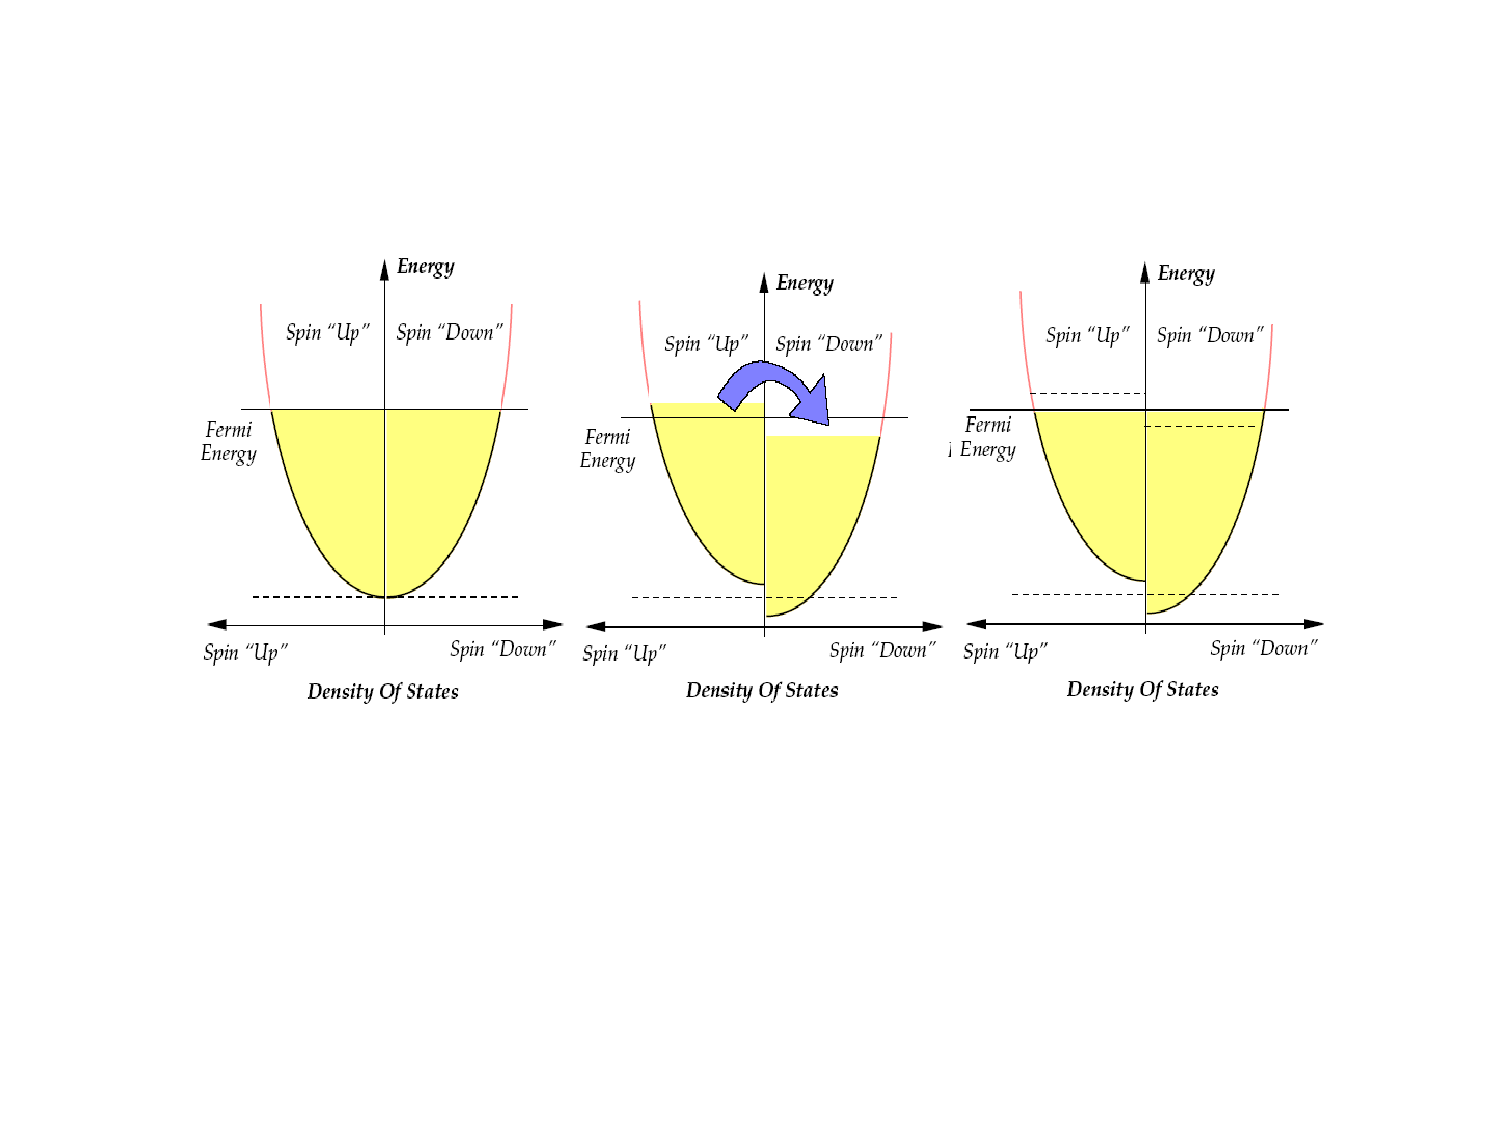
\includegraphics[width=0.8\linewidth]{paramag_fermi.pdf}
     \caption{自由电子自旋对于态密度的影响\label{fig:paramag_fermi}}
    \end{figure}
    \item 重新选取零点能使得 $\varepsilon = p^2/2m (+2\mu_BB)$ 代表自旋与磁场 (反) 平行的能量, 于是态密度
    \begin{equation}
        g(\varepsilon)\diff\varepsilon = \begin{cases}
            CV\sqrt\varepsilon\diff\varepsilon & 0\le\varepsilon\le 2\mu_BB\\
            CV\left(\sqrt\varepsilon + \sqrt{\varepsilon-2\mu_BB}\right)\diff\varepsilon & \varepsilon\ge 2\mu_BB
        \end{cases}
    \end{equation}
    其中 $C = 2\pi(2m)^{3/2}h^{-3}$, 与式(\ref{equ:state_density_for_ideal_gas}) 的区别在于分裂了自旋简并
    \item 磁场对 Fermi 能 $\mu_0$ 的影响: $0$K 时
    \begin{equation}
        N = \int_0^{\mu_0'}g(\varepsilon)\diff\varepsilon \Rightarrow
        \mu_0'^{3/2} + (\mu_0'-2\mu_BB)^{3/2} 
        = \frac{3N}{CV} = 2\mu_0^{3/2}
    \end{equation}
    通常磁场 $\mu_BB\ll\mu_0$ 时, $\mu_0' = \mu_0+\mu_BB$
    \item 磁化强度 $m$ ($0$K)
    \begin{equation}
        m = \frac 1V\left(\int_0^{\mu_0'}CV\sqrt\varepsilon\diff\varepsilon - \int_{2\mu_BB}^{\mu_0'}CV\sqrt{\varepsilon-2\mu_BB}\diff\varepsilon\right)\mu_B
        \approx C\mu_B^2\mu_0^{1/2}B
    \end{equation}
    带入 $\mu_0$ 式(\ref{equ:fermi_mu0}) 得到 $m = (3\mu_BB/2\mu_0)n\mu_B \ll n\mu_B$, 磁化率 $\chi_0 = 3n\mu_B^2/(2\mu_0)$, 不出现磁饱和
    \item 有限温 $T\ll T_F$ 时
    \begin{equation}
        \chi = \chi_0\left[1-\frac{\pi^2}{12}\left(\frac{T}{T_F}\right)^2 + O\left(\frac{T}{T_F}\right)^4\right]
    \end{equation}
    \item 高温时, 模型回到 \ref{sub:paramagnetic} 节的内容, 其中 $j=s=1/2$, $l=0$, $g=2$. 由式(\ref{equ:curie}) 得 %还需要补充!!!
    \begin{equation}
        m = \frac{\mu_B^2 nB}{k_BT}, \qquad \chi = \frac{n\mu_0\mu_B^2}{k_BT}
    \end{equation}
    注意: 上式中 $\mu_0$ 表示真空磁导率, 而非前文的 Fermi 能
    \begin{itemize}
        \item Landau 抗磁性: 
        带电粒子磁场中, 由于其轨通运动量子化而产生了抗磁性
        \item Van Leeuwen 定理: 广义动量 $p = mv + eA$ 对于结果的影响 (略)
    \end{itemize}
\end{enumerate}
% subsubsection paramagnetic_for_electron (end)
% subsection paramagnetic (end)
\subsection{负绝对温度} % (fold)
\label{sub:negtive_temperature}
\begin{enumerate}
    \item 内能越高, 可能的微观状态越少时, 出现负温度 
    $1/T = (\partial S/\partial U)_y < 0$
    \item 实现条件: 
    \begin{itemize}
        \item 系统能量有上界
        \item 系统内部实现平衡 (系统能与环境隔绝一段时间 / 系统本身弛豫时间远小于系统环境间平衡弛豫时间)
    \end{itemize}
    \item 二能级系统 $E = (N_+ - N_- )\varepsilon$, $S = k_B\ln\frac{N!}{N_+!N_-!}$
    \begin{equation}
        \frac 1T = \left(\frac{\partial S}{\partial E}\right)_\varepsilon
        = \frac{k_B}{2\varepsilon}\ln\left(\frac{N\varepsilon-E}{N\varepsilon+E}\right) = \frac{k_B}{2\varepsilon}\ln\frac{N_-}{N_+}
    \end{equation}
    当 $N_+>N_-$ 时出现负绝对温度
\end{enumerate}
% subsection negtive_temperature (end)
\subsection{气体吸附} % (fold)
\label{sub:gas_adsorption}
\begin{enumerate}
    \item 气体分子与被吸附分子单元两相平衡, 其中吸附项描述为
    \begin{itemize}
        \item 晶体表面有 $N_0$ 个等价固定位置可吸附分子, 被吸附分子与固体表面结合能 $\varepsilon_0$
        \item 被吸附分子数 $N\ll N_0$, 忽略它们间的相互作用
    \end{itemize}
    \item 气体分子, 半经典分布的理想气体, 式(\ref{equ:mu_semi_cla})
    \begin{equation}
        \mu' = -k_BT\ln\left[\frac{(2\pi m)^{3/2}(k_BT)^{5/2}}{ph^3}\right]
    \end{equation}
    \item 被吸附分子: 振动能与结合能 $E = E_v - N\varepsilon_0$. 配分函数
    \begin{equation}
        Z_N = \frac{N_0!}{N!(N_0-N)!}z_v^N\e^{N\beta\varepsilon_0}
    \end{equation}
    巨配分函数
    \begin{equation}
        \Xi = \sum_N \e^{-\alpha N}Z_N 
        = \left[1 + z_v\e^{-\alpha + \beta\varepsilon_0}\right]^{N_0}
    \end{equation}
    由平均粒子数以及$\alpha = -\beta\mu = -\beta\mu'$ 得到
    \begin{equation}
        \overline N = -\frac{\partial \ln\Xi}{\partial\alpha}
        = \frac{N_0}{1+z_v^{-1}\exp(\alpha -\beta\varepsilon_0)}
        = \frac{N_0p}{p+f(T)}
    \end{equation}
    \begin{itemize}
        \item 低压强 $p\ll f(T)$, $N = N_0 p/f(T)$, 与压强正相关
        \item 高压强 $p\gg f(T)$, $N = N_0$ 饱和
    \end{itemize}
    以上与实验定性符合, 定量不符, 因过于简化了.
\end{enumerate}
% subsection gas_adsorption (end)
% section model_independent (end)

\section{非近独立粒子的模型} % (fold)
\label{sec:model_non-independent}
\subsection{非理想气体物态方程} % (fold)
\label{sub:non-ideal_gas}
\begin{enumerate}
    \item 引入气体间势能, $E = E_t(p) + \Phi(q) + E_i$, 内部运动能量 $E_i$ 与 $(p,q)$ 无关. 
    \item 配分函数
    \begin{equation}
        Z = \frac 1{N!h^{3N}}\int\dif^{3N}p\,\e^{-\beta E_t}
        \int\dif^{3N}q\,\e^{-\beta\Phi}Z_i
    \end{equation}
    其中定义中间一项位形积分 $Q(\beta,V) = \int\dif^{3N}q\exp(-\beta\Phi)$
    \item 物态方程
    \begin{equation}\label{equ:vw_gas_p_origin}
        p = \frac 1\beta\frac{\partial\ln Z}{\partial V} 
        = \frac 1\beta\frac{\partial\ln Q}{\partial V}
    \end{equation}
    只考虑分子间两辆相互作用, 且分子势能只与分子间距有关, 即
    \begin{equation}
        \Phi = \sum_{1\le i< j\le N}U(r_{ij}) \equiv \sum \phi_{ij}
    \end{equation}
    一般的势能满足 $U(0) = \infty, U(\infty) = 0$, 
    引入分子接近程度的度量 $f_{ij}$
    \begin{equation}
        f_{ij} =f(r_{ij})\equiv \e^{-\beta\phi_{ij}}-1 
        \to \begin{cases}
            0     &r_{ij}\to\infty \\
            -1    &r_{ij}\to 0
        \end{cases}
    \end{equation}
    关于 $f_{ij}$ 展开 $Q$, 忽略多个分子两两相互接近即 $f{ij}$ 的二次及以上项
    \begin{align}
        Q &= \int\dif^{3N}q\prod_{i<j}(1+f_{ij}) \approx 
        \int\dif^{3N}q\left(1+\sum_{i<j}f_{ij}\right)\nonumber\\
        &= V^N + \frac 12 N(N-1)V^{N-2}\int\dif^3\vec R\int\dif^3\vec r f(r) 
        \approx V^N + N^2V^{N-1}a_2(T)
    \end{align}
    其中第二级 Virial 系数
    \begin{equation}
        a_2(T) = -\frac 12\int_\infty\dif^3\vec r f(r) 
        = -2\pi\int_0^\infty r^2\diff r\left(\e^{-\beta\phi(r)}-1\right)
    \end{equation}
    代入式(\ref{equ:vw_gas_p_origin}) 并保留到 $Na_2/V$ 的一阶, 得到物态方程
    \begin{equation}
        \frac{pv}{k_BT} = 1 + \frac{Na_2(T)}{v} \qquad v = \frac VN
    \end{equation}
    \begin{itemize}
        \item van der Waals 物态方程: 取分子间相互作用为 van der Waals 力
        \begin{equation}
            \phi(r) = \begin{cases}
                \infty        &r<r_0 \\
                -\mu r^{-6}   &r>r_0
            \end{cases}
        \end{equation}
        可以得到 $a_2(T) = b-a(T)/k_BT$, 于是
        \begin{equation}
            \frac{pv}{k_BT} = 1+\frac bv - \frac{a(T)}{k_BTv}
            \approx \frac{v}{v-b} - \frac{a(T)}{k_BTv}
        \end{equation}
        即 van der Waals 方程 $(p+a/v^2)(v-b) = k_BT$
    \end{itemize}
\end{enumerate}
% subsection non-ideal_gas (end)
\subsection{Ising 模型} % (fold)
\label{sub:ising_model}
\begin{enumerate}
    \item 试图解释铁磁性物质在 $T<T_c$ 时的自发磁化现象. 描述 $N$ 个各点, 各自取向 $S_i = \pm 1$, 对应微观状态 $\{S_i\}$, 以及能量
    \begin{equation}
        E\{S_i\} = -\sum_{\{ij\}}\varepsilon_{ij}S_iS_j - \mu_0\mu H\sum_i S_i
    \end{equation}
    其中 $\{ij\}$ 表示仅考虑最邻对的相互作用, $\mu_0\mu H$ 是磁场.
    \begin{itemize}
        \item 一维 (Ising), 二维 (Onsager) 均有严格解
        \item 各向同性介质 $\varepsilon_{ij} = \varepsilon$, 于是有基态
        \begin{itemize}
            \item[*] $\epsilon > 0$: $\cdots\uparrow\uparrow\uparrow\uparrow\uparrow\uparrow\uparrow\uparrow\uparrow\cdots $ 铁磁体
            \item[*] $\epsilon < 0$: $\cdots\uparrow\downarrow\uparrow\downarrow\uparrow\downarrow\uparrow\downarrow\uparrow\cdots $ 反铁磁体
        \end{itemize}
    \end{itemize}
    \item 配分函数与宏观量:
    \begin{align}
        &Z = \sum_{\{S_i\}}\exp\left[\beta\left(\varepsilon\sum_{\{ij\}} S_iS_j+ \mu_0\mu H\sum_i S_i\right)\right] \\
        &\overline E (H,T) = -\frac{\partial \ln Z}{\partial\beta} \\
        &C_H (H,T) = \left(\frac{\partial \overline E}{\partial T}\right)_H \\
        &M(H,T) = \mu\overline{\sum_i S_i} = \frac 1\beta \frac{\partial\ln Z}{\partial(\mu_0 H)}
    \end{align}
    当 $M(0,T)\neq 0$ 时称自发磁化, 铁磁性
    \item 平均场 (Bragg-Williams) 近似: 作用于 $S_i$ 的力 $\mu_0\mu H\sum_j\varepsilon_{ij}S_j$, 其等效磁场为
    \begin{equation}
        H_i = H + \frac 1{\mu_0\mu}\sum_j\varepsilon_{ij} S_j
    \end{equation}
    对上式取平均
    \begin{equation}
        \overline H_i = H + \frac 1{\mu_0\mu}z_0\varepsilon \overline S
    \end{equation}
    其中 $z_0$ 是给定格点的最近格点数量, 二维方阵中为 $2$, 三维简单立方中为 $6$, 体心立方为 $8$. 平均场近似即用 $\overline H$ 替代 $H_i$, 将相互作用自旋系统化为近独立自旋系统
    \begin{equation}
        Z = z^N \equiv \left(\e^{\beta\mu_0\mu\overline H} + \e^{-\beta\mu_0\mu\overline H}\right)^N
    \end{equation}
    据此得到 
    \begin{equation}
        M = \frac 1\beta\frac{\partial\ln Z}{\partial\mu_0 H} = N\mu\tanh\left(\frac{\mu_0\mu\overline H}{k_BT}\right) = N\mu\overline S
    \end{equation}
    若存在自发磁化, 则
    \begin{equation}
        \tanh\left(\frac{\varepsilon z_0\overline S}{k_BT}\right) = \overline S
    \end{equation}
    超越方程有非零解的条件 $\epsilon z_0/k_BT > 1$, 得到临界温度 $T_c = \epsilon z_0/k_B$. 
    \begin{itemize}
        \item 平均场近似的结果都显著的大于严格解的结果, 因为平均场忽略了涨落, 而涨落会破坏有序性
        \item  取序参量 $\overline S$, 上述模型可以变为 Landau 相变模型 (\ref{sub:landau_transi} 节)
    \end{itemize}
\end{enumerate}
% subsection ising_model (end)
% section model_non-independent (end)

\section{相变} % (fold)
\label{sec:phase_transition}
\subsection{热力学理论} % (fold)
\label{sub:phase_tra_thermo}
\begin{enumerate}
    \item 平衡条件: 以孤立系为例, 要求总熵取到极致 $\delta S = \delta S_\alpha + \delta S_\beta = 0$, 得到
    \begin{itemize}
        \item 热平衡条件: $T_\alpha = T_\beta$
        \item 力学平衡条件: $p_\alpha = p_\beta$
        \item 相变平衡条件: $\mu^{(i)}_\alpha = \mu^{(i)}_\beta$
    \end{itemize}
    \item 化学反应 $\sum \nu_i A_i = 0$, 
    等温等压下使 $G$ 极小, 即 $\sum \nu_i\mu_i = 0$
    \begin{itemize}
        \item $\sum \nu_i\mu_i <0$, 反应正向进行
        \item $\sum \nu_i\mu_i >0$, 反应逆向进行
    \end{itemize}
    \item Gibbs 相律: 对于 $k$ 种组元, $\varphi$ 个共存相, 体系的自由度 $f = k+2-\varphi$ (变量数$-$方程数). 进而有 $\varphi\le k+2$
    \item Ehrenfest 对相变的分类
    \begin{itemize}
        \item 一级相变: $y = \partial G/\partial Y$, $S = \partial G/\partial T$ 在相变点不连续. 
        \begin{itemize}
            \item 相变潜热 $\Delta H = T\Delta S$
        \end{itemize}
        \item 二级相变: 上述一阶导数连续, 而二阶导数不连续 (如热容不连续, BEC)
        \item 连续相变: 二级相变, 三级相变......
    \end{itemize}
\end{enumerate}
% subsection phase_tra_thermo (end)
\subsection{van der Waals 气体的相变} % (fold)
\label{sub:van_der_waals_trans}
根据 van de Waals 物态方程得到等温线 (图\ref{fig:vanderWaalsConstT})
\begin{equation}
    p = \frac{RT}{v-b} - \frac{a}{v^2}
\end{equation}
 \begin{figure}[!ht]
  \begin{minipage}[t]{0.5\linewidth}
    \centering
    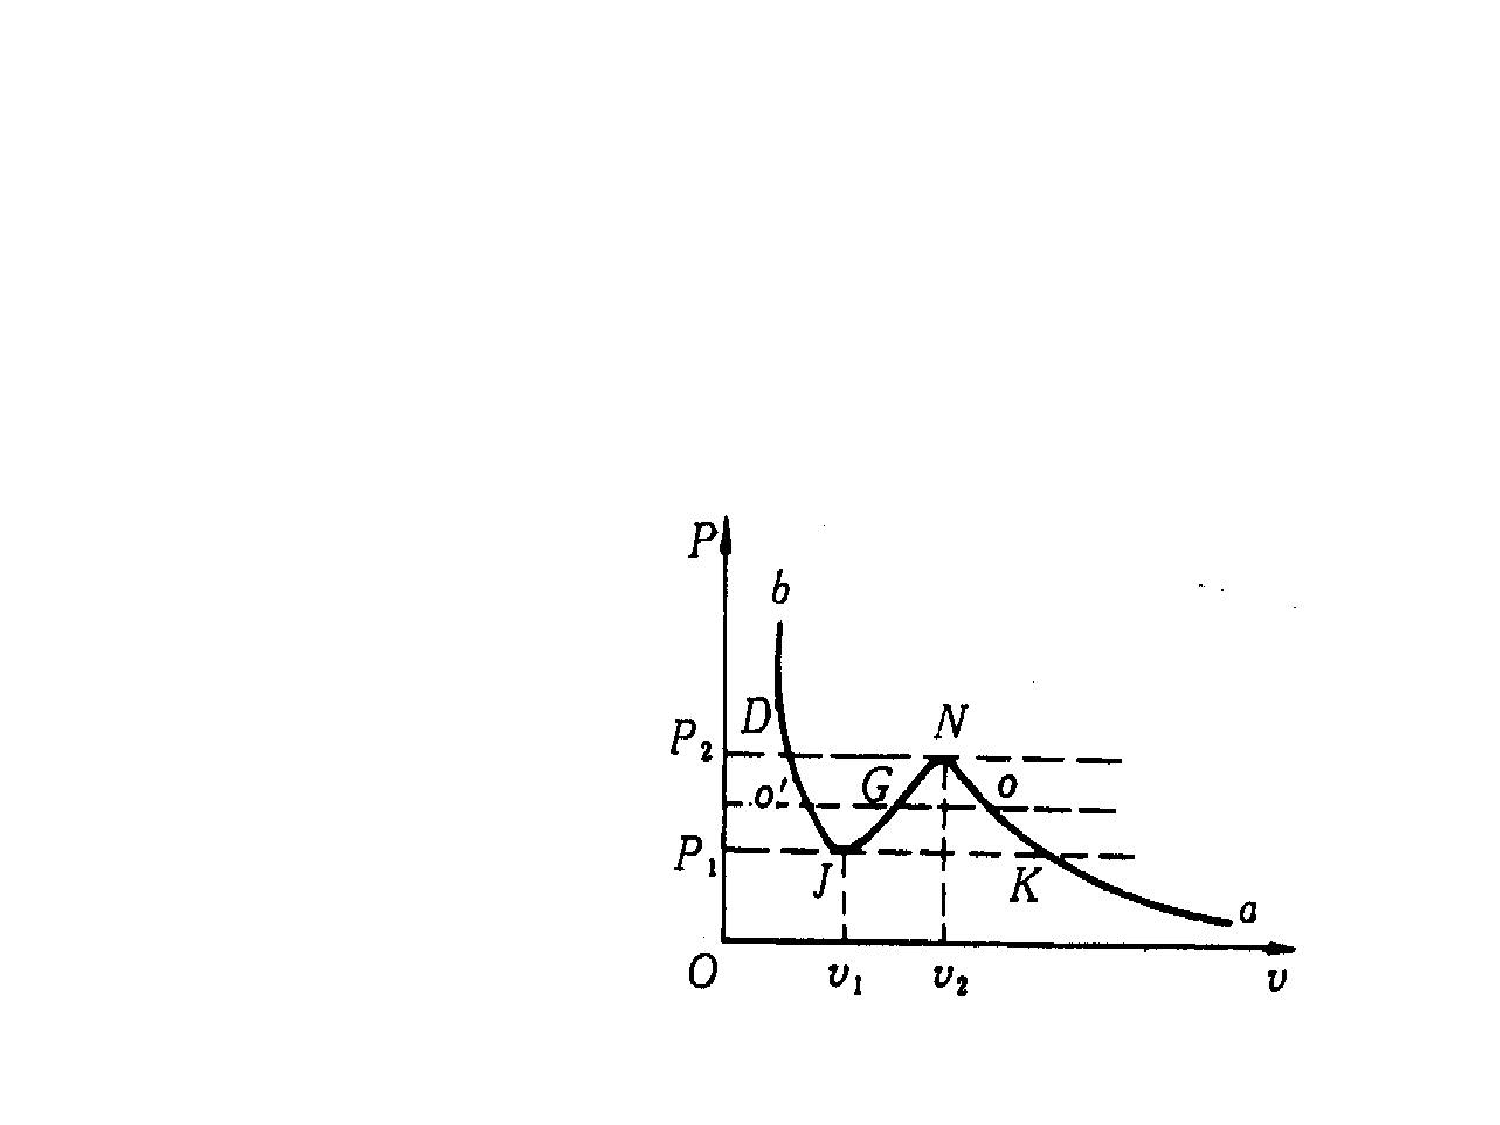
\includegraphics[width=0.9\linewidth]{vanderWaalsConstT.pdf}
    \caption{van der Waals 方程等温线\label{fig:vanderWaalsConstT}}
  \end{minipage}%
  \begin{minipage}[t]{0.5\linewidth}
    \centering
    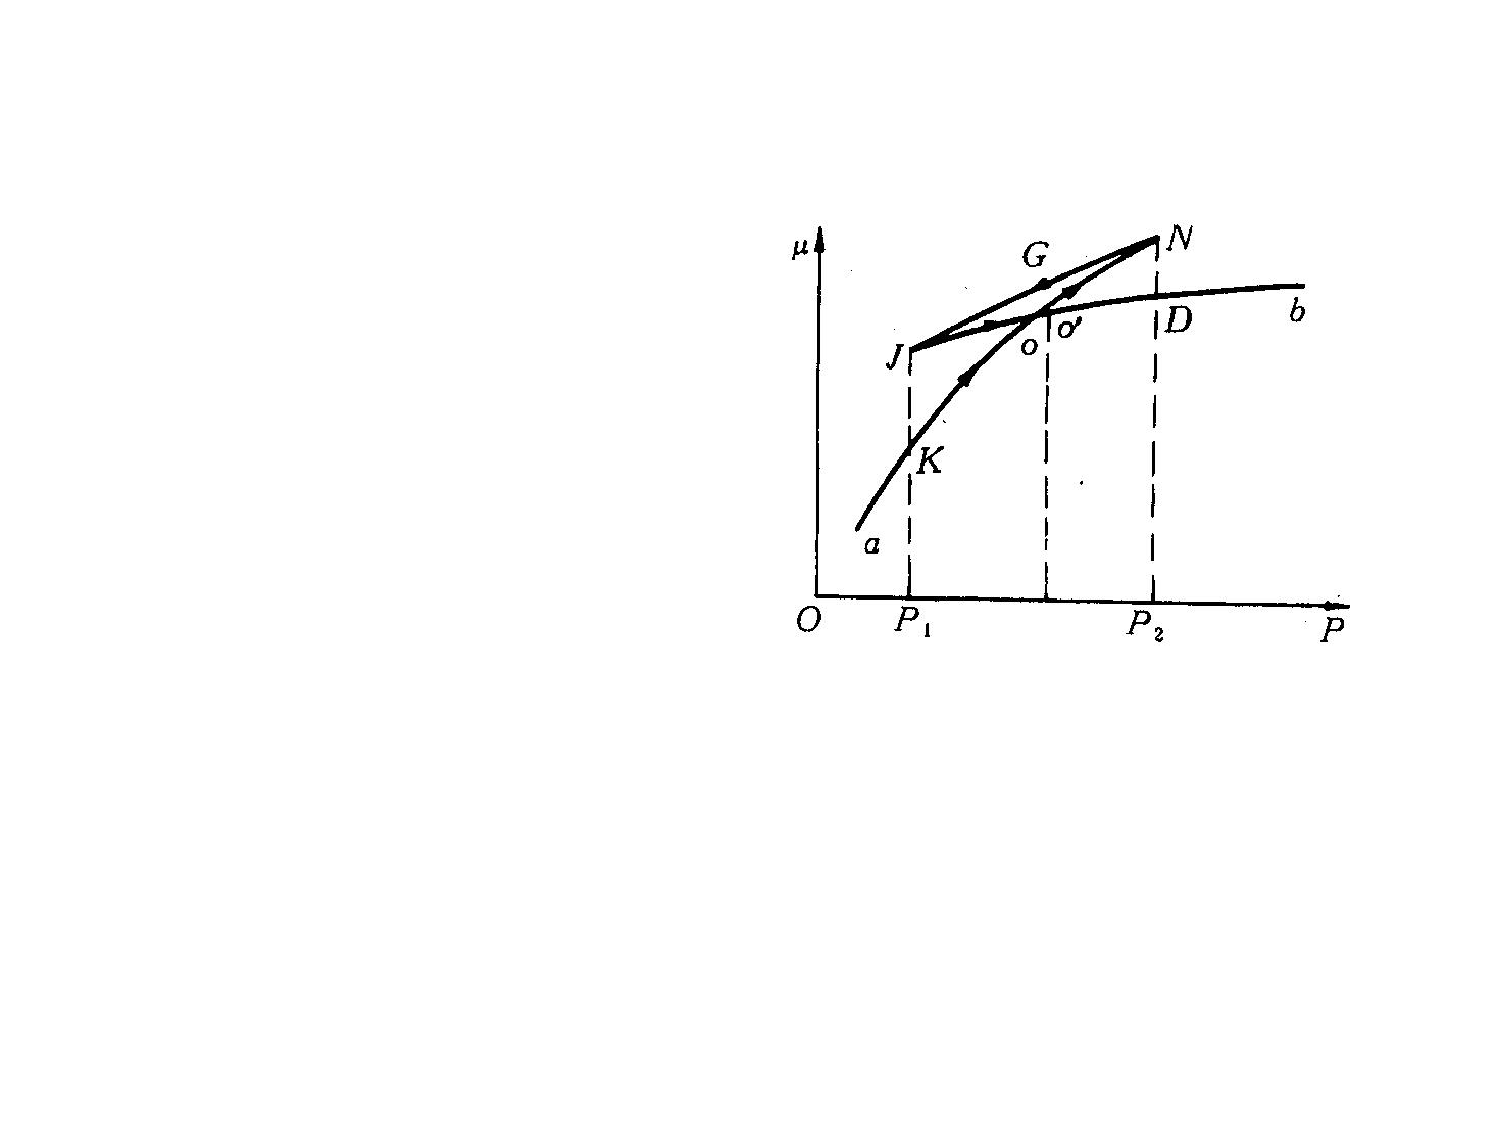
\includegraphics[width=0.9\linewidth]{vanderWaalsMu.pdf}
    \caption{van der Waals 化学势\label{fig:vanderWaalsMu}}
  \end{minipage}
  \end{figure}
其中 JN 段不稳定, 实际发生相变. 实际的稳定项由化学势确定
\begin{equation}
    \mu_m - \mu_0 = \int_{p_0}^p V_m\diff p
\end{equation}
据此找到 $\mu_{mo} = \mu_{mo'}$.

相变临界点: 等温线上原本的极大点和极小点重合为拐点, 即
\begin{equation}
    \left(\frac{\partial p}{\partial v}\right)_T = 0,\qquad 
    \left(\frac{\partial^2 p}{\partial v^2}\right)_T = 0
\end{equation}
据此解得
\begin{equation}
    T_c = \frac{8a}{27Rb},\qquad p_c = \frac{a}{27b^2},\qquad
    v_c = 3b,\qquad \frac{RT_c}{p_cv_c} = \frac 83 = 2.667
\end{equation}
定义对比参量 $x^*\equiv x/x_c$, 得到 van der Waals 对应态定律
\begin{equation}
    \left(p^* + \frac{3}{v^{*2}}\right)\left(v^*-\frac 13\right) = \frac 83 T^*
\end{equation}
% subsection van_der_waals_trans (end)
\subsection{Landau 相变理论} % (fold)
\label{sub:landau_transi}
\begin{enumerate}
    \item 序参量: 相变对应着物质有序程度的改变以及与之伴随的对称性的变化, 
    引入序参量 (对于 $m \leftrightarrow -m$ 对称) 描述有序程度, 在不同的相变中实际是不同的物理量
    \begin{itemize}
        \item 无序相: 序参量$= 0$; 
        有序相: 序参量$\neq 0$, 对称性破缺
        \item 序参量可以是一维标量, 也可以是多维的矢量 / 张量; 
        可以是实数, 也可以是复数 (超导, 超流)
    \end{itemize}
    \item 讨论连续相变在临界温度 $T = T_c$ 附近的行为 (临界现象)
    \item 临界指数, 描述临界点附近的奇异性 ($\Psi$ 为序参量, $J$ 为它的对偶场)
    \begin{align}
        &\chi \equiv \frac{\partial \Psi}{\partial J} = -\left(\frac{\partial^2G}{\partial J^2}\right)_T 
         \xlongequal{T\to T_c} \begin{cases}
            C\left(\frac{T}{T_c} - 1\right)^{-\gamma} &T>T_c \\
            C'\left(1 - \frac{T}{T_c}\right)^{-\gamma'} &T<T_c
        \end{cases}\\
        &C_J \equiv T\frac{\partial S}{\partial T} = -T\left(\frac{\partial^2G}{\partial T^2}\right)_{\Psi = 0} 
         \xlongequal{T\to T_c} \begin{cases}
            A\left(\frac{T}{T_c} - 1\right)^{-\alpha} &T>T_c \\
            A'\left(1 - \frac{T}{T_c}\right)^{-\alpha'} &T<T_c
        \end{cases}\\
        &\Psi_{T\to T_c} = B\left(1-\frac{T}{T_c}\right)^\beta \qquad
        \Psi_{T = T_c} = DJ^{1/\delta}
    \end{align}
    其中 $\alpha, \alpha', \gamma, \gamma', \beta, \delta$ 称为临界指数, $A, A', C, C', B, D$ 称为临界振幅. 
    铁磁系统中 $\Psi = M$ 为磁矩, $J = H$ 为磁场强度. 
    类似的在气液系统中, $\Psi = \Delta\rho$, $J = \Delta p$.\footnote{气液体系中关于临界指数的定义没弄明白...}
    \item 序参量密度 $m(\vec r)$: $M = \left\langle \int\dif^3\vec rm(\vec r)\right\rangle$, 粗粒平均...
    \item 关联函数 $\Gamma$ 与关联长度 $\xi$
    \item Landau 自由能的唯象理论:
    \begin{equation}
        F(m) = F_0(T) + \frac 12 a(T)m^2 + \frac 14b(T)m^4 + \cdots
    \end{equation}
    对于 $m \leftrightarrow -m$ 对称, 因而不含奇数次项. 稳定位置在 $F$ 取到极小值时. 若$\partial F/\partial m = 0$, $\partial^2 F /\partial m^2 > 0$ 存在非零解 $m\neq 0$, 则发生相变. 临界点为恰能发生相变的温度. 

    特别的, 取到 $m^4$ 项, 当 $a<0$ 时有三个解 $m = 0,\pm\sqrt{-a/b}$, 因而 $a(T_c) =0$. 设 $a = a_0(T/T_c-1)$, $b = \mbox{const.}$ 则得到临界点附近
    \begin{align}
        &m = 0 &(T>T_c) &\qquad& m = \pm\sqrt{\frac{a_0}{b}}\left(1-\frac{T}{T_c}\right)^{1/2} &(T<T_c) \\
        &C = -T\frac{\partial^2 F}{\partial T^2} = \frac{a_0^2}{2bT_c}
    \end{align}
    可见 $\beta = 1/2$, $\alpha = 0$. 在 $F$ 中加入外场 $-Bm$, 可以得到 $\delta = 3$, $\gamma = 1$
\end{enumerate}
% subsection landau_transi (end)
% section phase_transition (end)

\section{涨落} % (fold)
\label{sec:fluctuation}
\begin{enumerate}
    \item 绝对涨落 $\Delta X \equiv \sqrt{\overline{(X-\overline X)^2}} = \sqrt{\overline{E^2} - \overline E^2}$, 相对涨落 $\delta X = \Delta X/ \overline X$
    \item 封闭系统的能量涨落 $\Delta E =\sqrt{k_BT^2C_V}$
    \begin{align}
        \overline{E^2} &= \frac 1Z \frac{\partial^2 Z}{\partial \beta^2} = k_BT^2C_V + \overline E^2
    \end{align}
    对于单原子分子理想气体 $\delta E = \sqrt{2/3N} \sim 10^{-11}$
    \item 开放系统的能量涨落与粒子数涨落
    \begin{equation}
        \frac{\Delta E^2}{\overline E^2} = \frac{kT^2C_V}{\overline E^2} + \frac{\Delta N^2}{\overline E^2}\left(\frac{\partial E}{\partial N}\right)_{T,V}^2
    \end{equation}
    对于单原子分子理想气体 $\Delta N = 1/\sqrt{\overline N}$, $\delta E = \sqrt{5/3\overline N}$
\end{enumerate}
通常情况下相对涨落极小, 此时系统基本处于均值状态, 三种系统等价. 临界点附近涨落大
% section fluctuation (end)

\section{非平衡统计力学} % (fold)
\label{sec:non-equilibrium_SM}
基于分布函数 $f(\vec r,\vec v, t)\diff^3 \vec r\dif^3\vec v$ 讨论经典钢球模型. 常用的理想气体平衡态 Maxwell 分布
\begin{equation}
    f = n\left(\frac m{2\pi k_B T}\right)^{3/2}\exp\left(-\frac {m\vec v^2}{2k_B T}\right)
\end{equation}

对于两个分子相互关联, 常用到\emph{分子混沌假设}
\begin{equation}
    f(\vec r,\vec v_1,\vec v_2,t) \cong f_1(\vec r,\vec v_1,t)f_2(\vec r,\vec v_2, t)
\end{equation}
\subsection{分子碰撞} % (fold)
\label{sub:molecule_collision}
\begin{enumerate}
    \item 碰壁数 $\Gamma$: 
    单位时间内碰到单位面积容器壁上的分子数
    \begin{equation}
        \Gamma(\vec r, t) = \int\dif^3\vec v v_xf(\vec r,\vec v, t)
    \end{equation}
    对于 Maxwell 分布, $\Gamma = \frac 14 n\overline v$
    \item 碰撞频率
    \begin{align}
        &\theta_{12}(\vec r,\vec v_1,t) = \pi\left(\frac{\sigma_1+\sigma_2}2\right)^2\int\dif^3\vec v_2|\vec v_2 - \vec v_1|f_2(\vec r,\vec v_2,t) \\
        &\theta_{12}(\vec r,t) = \frac{\int\dif^3\vec v_1\theta_{12}(\vec r,\vec v_1,t)f_1(\vec r,\vec v_1,t)}{\int\dif^3\vec v_1 f_1(\vec r,\vec v_1,t)}
    \end{align}
\end{enumerate}
% subsection molecule_collision (end)
\subsection{Boltzmann 输运方程} % (fold)
\label{sub:boltzmann_equ}
\begin{enumerate}
    \item 稀薄气体近似: 分子短时碰撞, 碰撞外是自由的 (高温低密), 于是
    \begin{equation}
        \frac{\partial f}{\partial t} = \left(\frac{\partial f}{\partial t} \right)_{\mathrm{drift}} + \left(\frac{\partial f}{\partial t} \right)_{\mathrm{collision}}
    \end{equation}
    \begin{itemize}
        \item 漂移项
        \begin{equation}
            \left(\frac{\partial f}{\partial t} \right)_{\mathrm d} = -\vec v\cdot\nabla_r f - \nabla_v \cdot(f\vec a) \stackrel*= -\vec v\cdot\nabla_r f - \vec a\cdot\nabla_v f
        \end{equation}
        $*$: $\nabla_v\cdot \vec a = 0$, 即作用力与速度无关或者 Lorentz 力
        \item 碰撞项 (要求钢球碰撞模型和分子混沌假设)
        \begin{equation}
            \left(\frac{\partial f}{\partial t} \right)_{\mathrm c} = \int_{\theta\in[0,\pi/2]}\dif\Omega\int\dif^3\vec v_1(f'f'_1 - ff_1)\Lambda
        \end{equation}
        其中 $\Lambda \equiv |\vec v - \vec v_1|\sigma^2\cos\theta$, $f_{(i)}^{(j)} \equiv  f(\vec r,\vec v_{(i)}^{(j)}, t)$, $\vec v'$ 表示碰撞后速度
        \begin{align*}
            \vec v' &= \vec v + [(\vec v_1 -\vec v)\cdot\vec n]\vec n \\
            \vec v_1' &= \vec v_1 + [(\vec v -\vec v_1)\cdot\vec n]\vec n
        \end{align*}
    \end{itemize}
    两项加入
    \begin{equation}
        \frac{\dif f}{\dif t} = \frac{\partial f}{\partial t} + \vec v\cdot\nabla_r f + \vec a\cdot\nabla_v f = \iint\dif\Omega\dif^3\vec v_1(f'f'_1 - ff_1)\Lambda
    \end{equation}
    推广到多组分的情形 ($\Lambda_{ij} \equiv |\vec v - \vec v_1|(\sigma_i + \sigma_j)^2\cos\theta /4 $)
    \begin{equation}
        \frac{\dif f_i}{\dif t} = \sum_j\iint\dif\Omega\dif^3\vec v_1(f_i'f'_{j1} - f_jf_{i1})\Lambda_{ij}
    \end{equation}
    定义 $\Lambda = \dif\Sigma/\dif\Omega$ 为微分散射截面, 则不限于钢球碰撞模型. \\
    去掉分子混沌假设, 则需要将 $f'f'_1 , ff_1$ 替换为关联分布, 求解设计 BBGKY Hierarchy
\end{enumerate}
% subsection boltzmann_equ (end)
\subsection[Boltzmann H 定理]{Boltzmann $H$ 定理} % (fold)
\label{sub:boltzmann_h_theorem}
\begin{enumerate}
    \item $H$ 函数, 分布函数 $f(\vec r,\vec v, t)$ 的泛函
    \begin{equation}
        H(t) \equiv \int\dif^3\vec r\dif^3\vec v f(\vec r,\vec v, t)\ln f(\vec r,\vec v, t)
    \end{equation}
    \item Boltzmann $H$ 定理: 若 $f(\vec r,\vec v, t)$ 满足输运方程, 则
    \begin{equation}
        \frac{\dif H (t)}{\dif t}\le 0
    \end{equation}
    取等号当且仅当 $f'f_1 = ff_1$. 具体来说, 漂移项贡献为 $0$, 碰撞项贡献
    $$
    \frac{\dif H (t)}{\dif t} = -\frac 14 \int\dif^3\vec r\dif^3\vec v'\dif^3\vec v_1\dif\Omega\left[\ln(f'f_1')-\ln(ff_1)\right]\left[f'f_1' - ff_1\right]\Lambda
    $$
    \item $H$ 函数与熵: $S = -k_B H + \mbox{conts.}$
    \begin{itemize}
        \item 对于任意态都可以定义 $H$, 但热力学熵仅对平衡态有定义
        \item 熵增原理适用于任意孤立体系, $H$ 定理成立要求 $f$ 满足输运方程
        \item $H$ 定理给出了系统趋向于平衡态的速度
    \end{itemize}
    \item $H$ 定理是统计性的, 与微观的可逆性, Poincar\'e 之间的佯谬应用统计性质来解释
\end{enumerate}
% subsection boltzmann_h_theorem (end)
\subsection{细致平衡原理} % (fold)
\label{sub:detailed_balance}
平衡时, 每一个元过程都与它相应的逆过程相抵消. (并非普适)
\begin{enumerate}
    \item 细致平衡条件: $H$ 定理中达到平衡的条件
    \begin{equation}
        ff_1 = f'f_1'
    \end{equation}
    此时有输运项和碰撞项均为 $0$
    \item 平衡态的分布函数
    \begin{equation}
        f = n\left(\frac m{2\pi k_B T}\right)^{3/2}\exp\left[-\frac {m}{2k_B T}(\vec v-\vec v_0)^2\right]
    \end{equation}
    来源于细致平衡条件 $\ln f + \ln f_1 = \ln f' + \ln f_1'$ 的守恒与线性, 考虑碰撞的收衡量 ($\vec p$, $E_k$), 从而要求一般解为
    $$
     \ln f = c_1 p_x + c_2 p_y + c_3 p_z + c_4 E_k + c_5
    $$
    改变常数组得到上面的分布 (各参数应与 $\vec v$ 无关, 但可以依赖于 $r$), 此外为使 $\partial f/\partial t = 0$, 要求漂移项为 $\forall \vec v.\quad -\vec v\cdot\nabla_r f - \vec a\cdot\nabla_v f = 0$, 得到
    \begin{align}
        &\nabla_r \frac 1T = 0 
        &\Rightarrow& T = \mbox{const.}\\
        &\vec v\cdot\nabla_r(\vec v\cdot\vec v_0) = 0 
        &\Rightarrow& \vec v_0 = \vec \alpha + \vec\omega\times \vec r \\
        &\nabla_r\left(\ln n - \frac{mv_0^2}{2k_B T}\right) = \frac{m\vec a}{k_B T} 
        &\Rightarrow& n=n_0\exp\left(\frac{mv_0^2}{2k_BT} - \frac{U(\vec r)}{k_BT}\right) \\
        &\vec a \cdot\vec v_0 = 0
    \end{align}
\end{enumerate}
% subsection detailed_balance (end)
% section non-equilibrium_SM (end)
\appendix
\renewcommand\thesection{\Alph{section}}
\begin{multicols}{2}
\section{数学公式} % (fold)
\label{sec:math}
\begin{enumerate}
    \item Stirling 公式
    \begin{equation}
        n! \approx \sqrt{2\pi n}\left(\frac n\e\right)^n
    \end{equation}
    \item 二项式分布
    \begin{equation}
        P_N(n) = \frac{N!}{n!(N-n)!}p^n(1-p)^{N-n}
    \end{equation}
    \begin{enumerate}
        \item Poisson 分布: $N\gg 1, p\ll 1, \overline n = Np$
        \begin{equation}
            P_N (n) = \frac{\overline n^n}{n!}\e^{-\overline n}
        \end{equation}
        \item Gaussian 分布: $N\gg 1, p\sim 1-p$, 在 $\overline n = Np$ 极大附近, 方差 $\sigma^2 = Np(1-p)$
        \begin{equation}
            P_N = \frac1{\sqrt{2\pi\sigma^2}}\e^{-\frac{(n-\overline n)^2}{2\sigma^2}}
        \end{equation}
    \end{enumerate}
    \item Gaussian 积分
    \begin{align}
        &\int_{-\infty}^\infty\e^{-ax^2}\diff x = \sqrt{\frac{\pi}{a}} \\
        &\int_0^\infty x^n \e^{-ax^2}\diff x = \frac{\Gamma[(n+1)/2]}{2a^{(n+1)/2}}
    \end{align}
    \item Bose 分布中的积分公式
    \begin{align}
        \int_0^\infty\frac{x^{n-1}}{\e^x - 1} \diff x
        &= \Gamma(n)\sum_{k=1}^\infty\frac 1{k^n} \label{equ:bose}
    \end{align}
    其中 Riemann zeta 函数
    \begin{equation}
        \zeta (n) \equiv \sum_{k=1}^\infty\frac 1{k^n}
    \end{equation}
    上面用到的
    \begin{align}
        \zeta(3/2) &= 2.612 & \zeta(4) &= \pi^4/90 \\
        \zeta(5/2) &= 1.341
    \end{align}
    \item Fermi 分布中的积分公式
    \begin{equation}\label{equ:fermi}
        \int_0^\infty\frac{x^{2l}\e^x}{(\e^x+1)^2}\diff x 
        =\sum_{n=1}^\infty (-)^{n+1}n\frac{\partial^{2l}}{\partial n^{2l}}\frac 1n
    \end{equation}
    特别的 $l=1$ 时取到 $\pi^2/6$
    \item $n$ 维球体
    \begin{equation}
        I_n = \frac{\pi^{n/2}}{\Gamma(n/2+1)}R^n
    \end{equation}
\end{enumerate}
% section math (end)
\section{热力学关系} % (fold)
\label{sec:ThermoD}
\begin{enumerate}
    \item 特性函数及基本关系
    \begin{itemize}
        \item 熵 $S = k_B\ln\Omega$
        \begin{equation}
            \dif S = \frac 1T\dif U + \frac pT\dif V - \frac \mu T\dif N
        \end{equation}
        \item 内能 $U = E$
        \begin{equation}
            \dif U = T\dif S - p\dif V + \mu\dif N
        \end{equation}
        \item 焓 $H = U + pV$
        \begin{equation}
            \dif H = T\dif S + V\dif p + \mu\dif N
        \end{equation}
        \item Helmholtz 自由能 $F = U - TS$
        \begin{equation}
            \dif F = -S\dif T - p\dif V + \mu\dif N
        \end{equation}
        \item Gibbs 自由能 $G = F+pV$
        \begin{equation}
            \dif G = -S\dif T + V\dif p + \mu\dif N
        \end{equation}
        \item 巨热力学势 $J = F- \mu N$
        \begin{equation}
            \dif J = -S\dif T - p\dif V - N\dif \mu
        \end{equation}
    \end{itemize}
    \item Nernst 定理: 等温过程的熵变在零温极限下为 $0$
    \begin{equation}
        \lim_{T\to 0}\left(\Delta S\right)_T = 0
    \end{equation}
    Nernst 原理: 不可能使一个物体冷却到 $0$K%待补充
\end{enumerate}
% section ThermoD (end)
\end{multicols}
\end{document}
